\documentclass[11pt,french,a4paper]{report}
\usepackage[frenchb]{babel}
\usepackage[utf8]{inputenc}
\usepackage[left=2cm,right=2cm,top=2cm,bottom=2cm]{geometry}
\geometry{a4paper}
\usepackage{graphicx}
\usepackage{listings} 

\lstdefinestyle{customc}{
  belowcaptionskip=1\baselineskip,
  breaklines=true,
  frame=L,
  xleftmargin=\parindent,
  language=C,
  showstringspaces=false,
  basicstyle=\footnotesize\ttfamily,
}

\lstset{escapechar=@,style=customc}


\title{Rapport de Stage fin de DUT - SuperBeeLive}
\author{Olivia SERENELLI-PESIN}

\begin{document}

\maketitle

\clearpage
\newpage 

\chapter*{Remerciements}

J’adresse mes remerciements aux personnes qui m’ont permis de réaliser ce stage dans l’équipe de SuperBeeLive. \\
Tout d’abord Matthieu ROUSSET, initiateur du projet SuperBeeLive à l'IBMM (Insitut Biomoléculaire Max Mousseron) 
qui m’a accueilli au sein de son équipe. \\
Ensuite, Capucine CARLIER pour son accueuil, pour ses nombreuses explications biologiques sur les abeilles ainsi que sa disponibilité 
afin de comprendre au mieux les enjeux et les besoins des biologistes pour mon projet. \\
Enfin, Sebastien DRUON pour m’avoir encadré, aidé à m’intégrer dans le milieu de la recherche et aidé sur une multitude 
de sujets, aussi bien du point de vu universitaire que sur les tâches qui m’ont été confiées. \\

\tableofcontents

\clearpage

\chapter{Introduction : Présentation du projet de recherche}
\section{La structure d'accueil} 

Le projet étant réalisé par plusieurs laboratoires de recherches, j'ai dû évoluer au seins de différentes organisations. 
Tout d'abord il y a mon employeur, l'Université de Montpellier, qui englobe d'autres structures où j'ai pu évoluer. 
L'université a été, pour moi, une entitée administrative. \\ 
Avec elle, le CNRS (Centre National de Recherche Scientifique) accueille dans ses locaux le rucher expérimental où 
l'équipe peut effectuer ses tests d'installation pour le projet. J'ai pu m'y rendre plusieurs fois afin d'observer les abeilles
et voir l'installation évoluer au fur et à mesure. C'est également chez eux que nous aurons un serveur d'installé dans leur salle dédiée.\\
Ensuite, l'IBMM est le laboratoire qui a engagé l'argent lié au projet afin de pouvoir me recrutrer lors de ce stage. 
C'est également une structure qui a été seulement administrative de mon point de vu puisque j'ai été affectée dans 
les bureaux du LIRMM (Laboratoire d'informatique, de robotique et de microéléctronique de Montpellier), autre laboratoire de 
recherche, afin que je puisse être aux côtés de Sébastien DRUON qui m'aura donné la grande majorité de mes tâches à effectuer. 
J'ai pu y avoir mon bureau en face du siens, me permettant d'être autonome mais aussi de pouvoir faire
appel à lui facilement lorsque j'en avais besoin.\\
\\
C'est dans ce contexte de recherche que j'ai pu découvrir et travailler sur le projet SuperBeeLive. \\ 


\section{Le projet SuperBeeLive}
\subsection{Explication et intentions du projet}
 
La santé et le développement des abeilles est aujourd’hui une question de plus en plus étudiée. Les bouleversements
majeurs de notre planète et de l’activité humaine se traduisant par une augmentation alarmante de la mortalité
des colonies et une chute de la production du miel dans nos pays développés, il est urgent de se préoccuper de leur futur. 
La situation des abeilles domestiques alerte le pouvoir public sur l’accélération de la dégradation de la biodiversité des 
pollinisateurs domestiques et sauvages, et de la flore qui en dépend. Ces dégâts sont dûs, entre autre, à l’apparition 
et la prolifération d’espèces invasiges pour les abeilles, provoquant maladies et déteriorations. 

Le projet consiste en la structuration de plusieurs collaborations existantes ou nouvelles autours du developpement 
d’une ruche plate instrumentée destinée au monitorage détaillé de la santé de l’abeille et des écosystèmes. Son but est de
pouvoir répondre à des questions clés, notamment autours des mécanismes physiopathologiques et des maladies chroniques 
dûes au parasites ainsi qu’aux altérations de l’écosystèmes et des qualités nutritives des produits des ruches. \\
Répondre à ces questions permettra de regrouper différentes solutions technologiques systèmatiques, 
automatiques et non invasives à la collection de données usuelles déterminantes dans chacun des thèmes abordés.
Les différents travaux déjà effectués autours de ce sujet ne visaient qu’un seul type de problème à la fois, 
ne permettant pas une vision globale des difficultées rencontrées par les abeilles. Notre but est de réunir les différentes
données qui peuvent être utilisés pour étudier l’influence des éléments et événements extérieurs sur leur santé et leur cadre de vie.\\

Concrétement, l'équipe de SuperBeeLive va concevoir une ruche plate afin d'y mettre en place plusieurs type de capteurs
(hygrométrie, vibrations, température interne et externe, etc) ainsi que des caméras qui filmeront l'intérieur et 
l'extérieur de la ruche. \\
En 2017, une affiche résumant le projet a été présentée lors du salon NUMEV (Solutions, Numériques, Matérielles, et 
Modélisation pour l'Environnement et le Vivant) (Annexe 1). \\ 
%TODO mettre lien avec annexe (affiche 2017) 

\begin{figure}[!h]
\centering
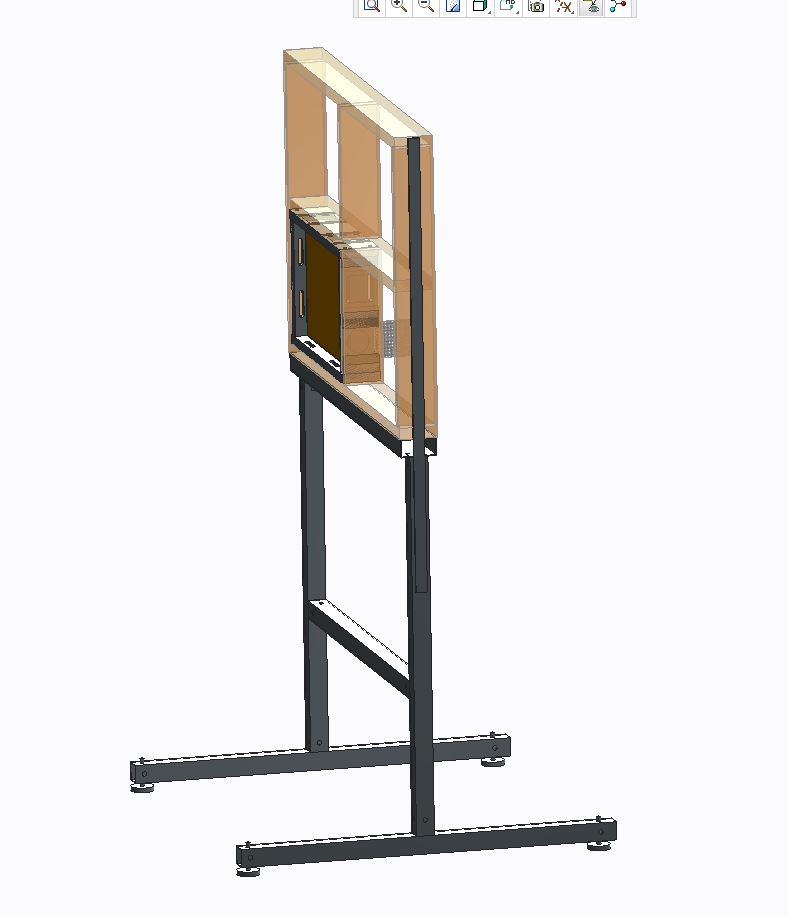
\includegraphics[scale=0.3]{../images/schema_ruche/supportrucheplate1.JPG}
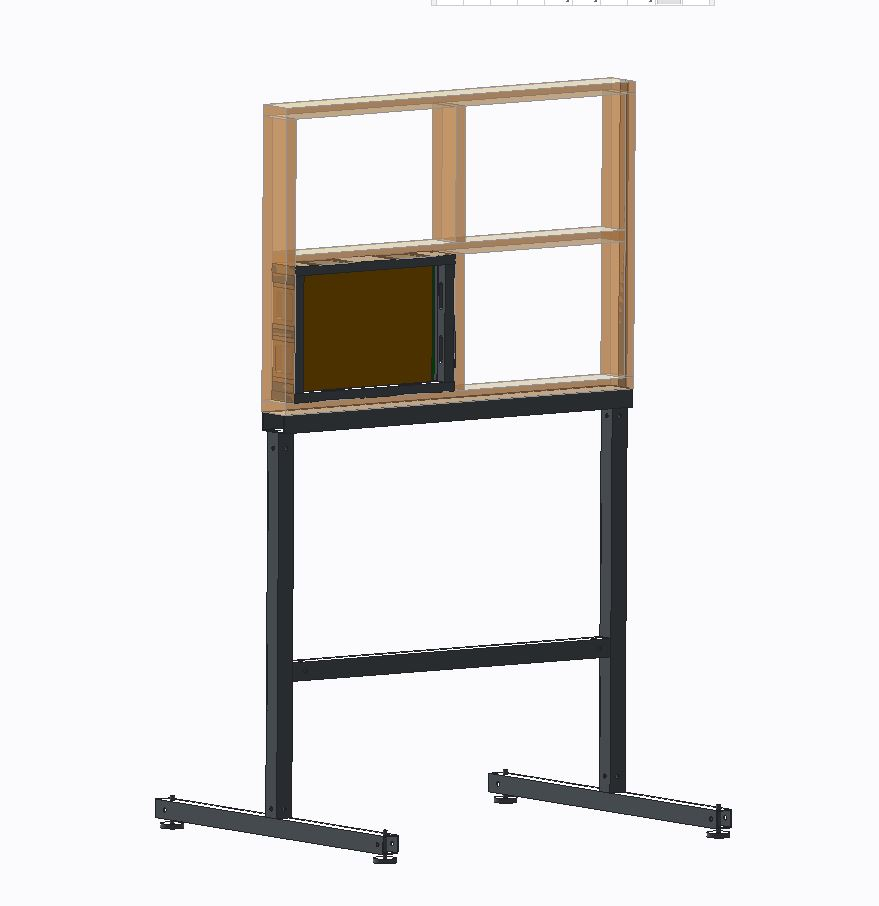
\includegraphics[scale=0.3]{../images/schema_ruche/supportrucheplate.JPG} 
\caption{Schéma de la ruche plate}
\label{schema_conception}
\end{figure}

\begin{figure}[!h]
\centering
\includegraphics[scale=0.05,angle=270]{../images/photo/face_ruche.jpg}
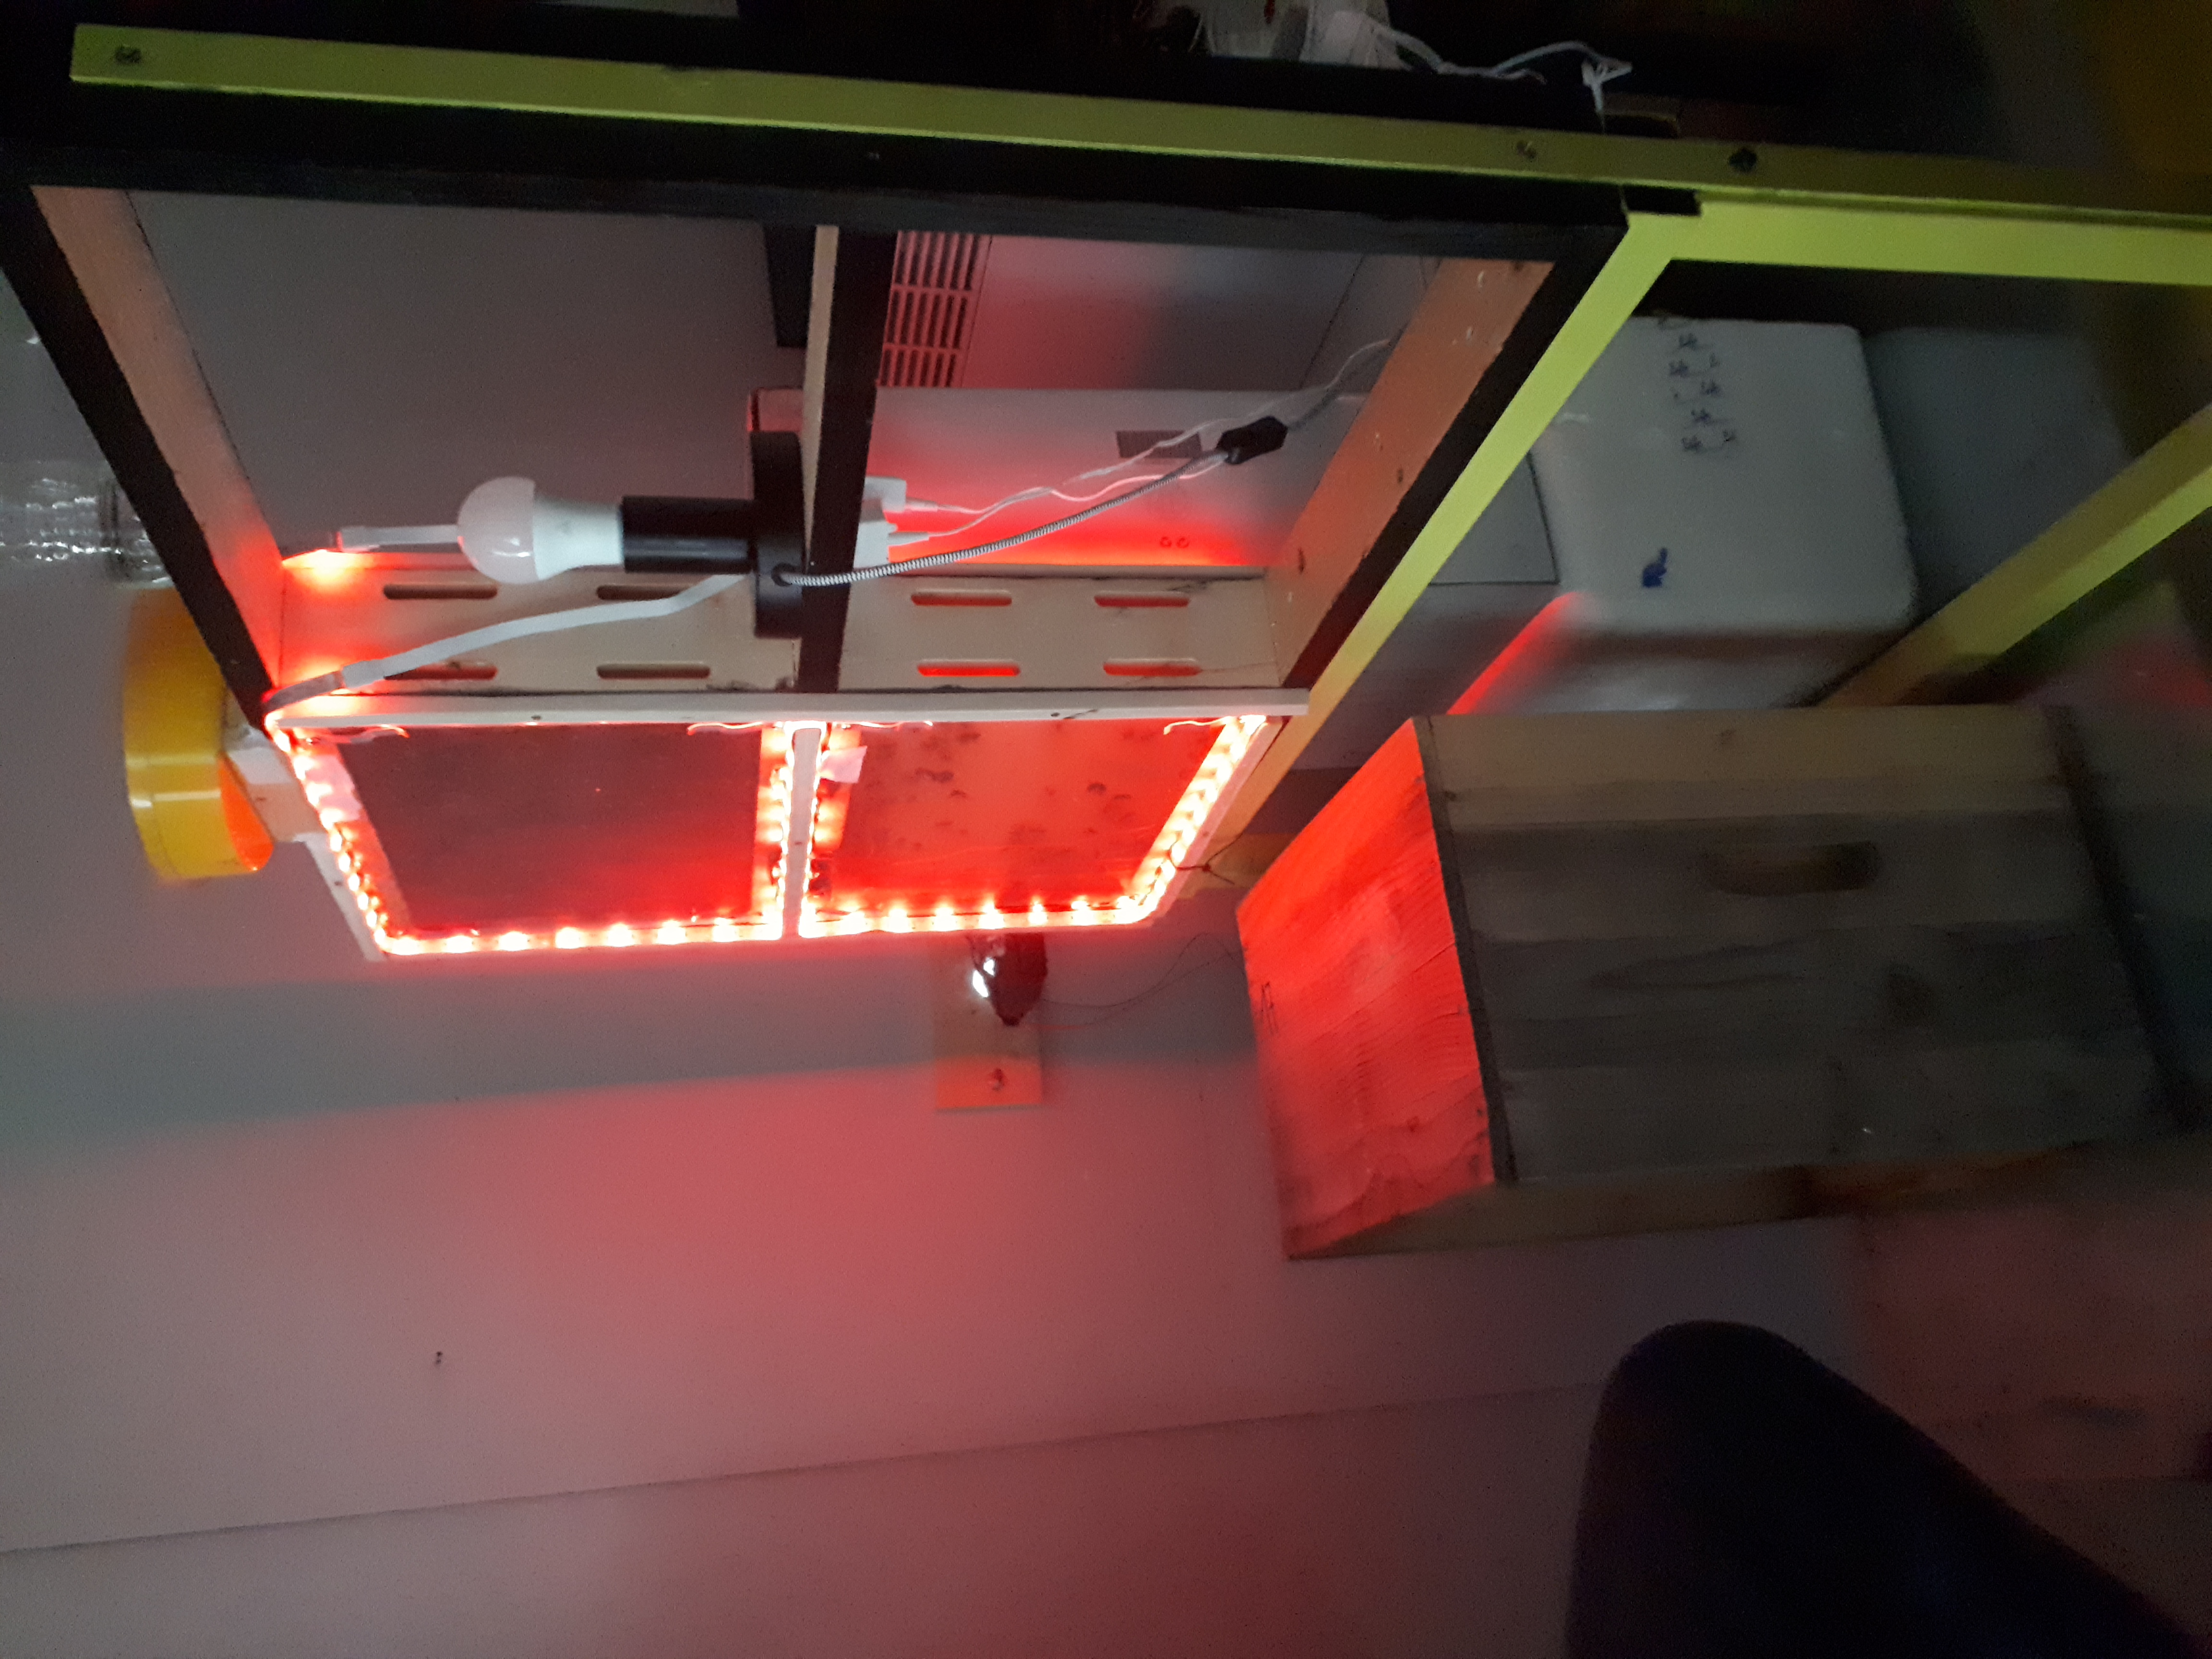
\includegraphics[scale=0.05,angle=270]{../images/photo/cote_ruche.jpg} \\
\caption{Photos de la ruche plate à mon arrivée}
\label{photo_rucher}
\end{figure}

Dans un premier temps, cette instrumentation nous permettra d'observer en temps réel la ruche et ses habitantes : 
les caméras nous donnerons une vision globale de ce qu'il s'y passe, aussi bien en intérieur pour observer leur 
comportement et tenter de repérer des parasites comme le varoa, qu'en extérieur pour y voir les dangers comme le frelon asiatique. %TODO REF ASIATIQUE ET VAROA  
Couplée aux donnés récoltées à l'aide de la carte éléctronique et ses capteurs installée au centre de la ruche plate, 
nous pourrons avoir une vision complète et détaillées des événements et leur répercutions ponctuant la vie d'une colonie,
de sa naissance à sa mort. \\
Ces observations ont pour but d'être enregistrée, sauvegardées et commentées par les biologistes afin de construire une base
de donnée contenant plusieurs types de comportements comme le refroidissement de la ruche, les danses frétillante %TODO REF DANSE 
\\
Dans un second temps, cette base de donnée pourra être utilisée afin de créer des algorithmes repérant ces différents comportement
de manière automatisée. Cela nous permettrait, en plus d'avoir des données complètes et utilisables, d'en avoir leur analyse en 
temps réel. Ces informations seront diffusées de deux façon. D'abord, elles seront partagées pour être étudiées par d'autres scientifiques, 
notamment les colaborateurs autours du projet SuperBeeLive. Ensuite, Le projet se veut aussi éducatif : une vitrine Web accessible au public 
sera créée présentant une ruche et ses données numériques et vidéos commentées en live. \\

Ainsi, les ruches plates de SuperBeeLive permetront de fournir des données crutiales pour des futures recherches autours des abeilles, tout en 
éduquant le grands public à l'importance des abeilles et les risques liées à nos activités humaines pour cette espèces et la biodiversité. 

\section{L'équipe}
L'équipe de recherche qui constitue le projet SuperBeeLive est répartie entre plusieurs laboratoires, je n'ai donc pas eu l'occasion
d'en rencontrer tous les acteurs, certains se trouvant même à l'étranger. Voici un schéma représentant globalement la structure
de l'équipe ainsi que les membres avec qui j'ai pu travailler. \\

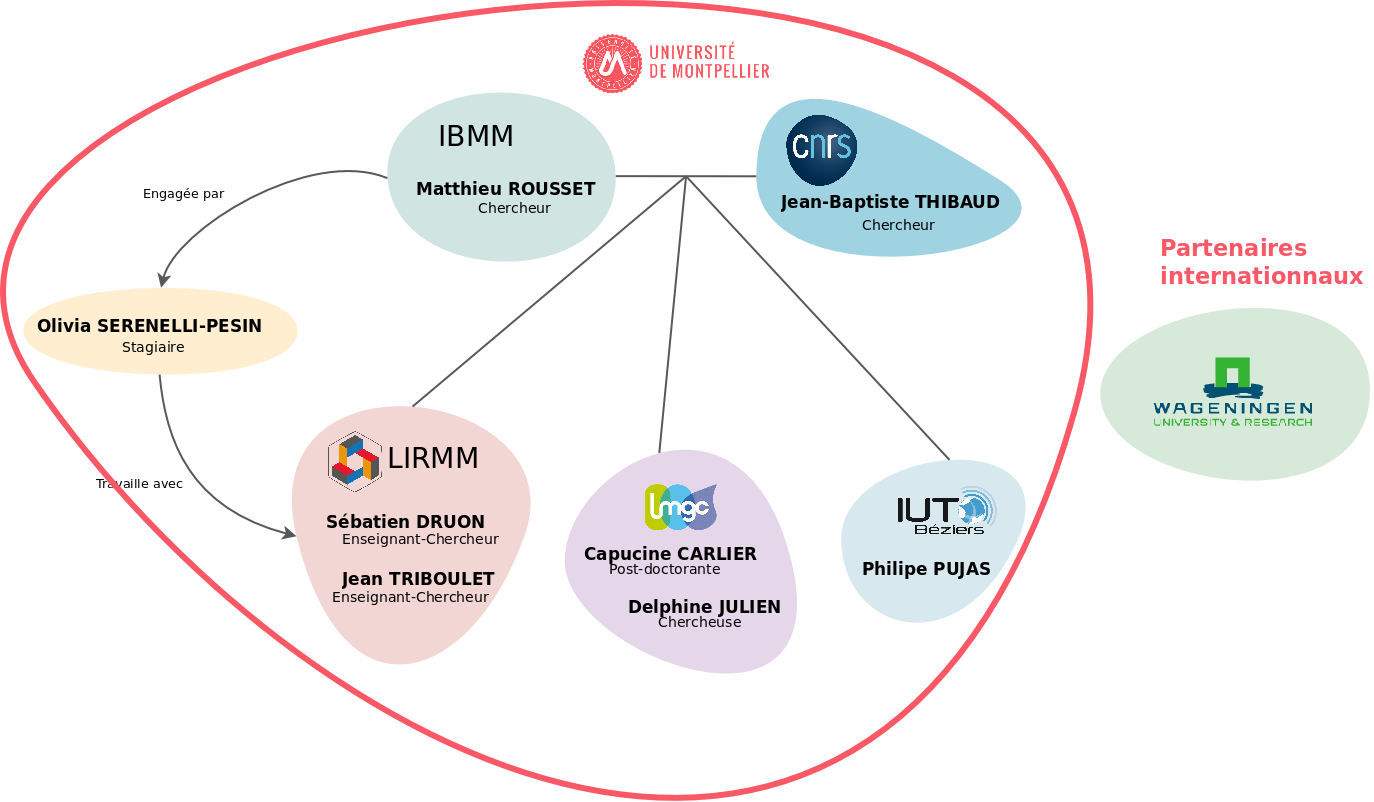
\includegraphics[scale=0.3]{../images/dia/organiramme_equipe_projet.png} \\

Les laboratoires de recherche principaux sont l'IBMM (Institut Biomoléculaire Max Mousseron) 
et le CNRS (Centre National de la Recherche Française) représentés ici respectivement par Matthieu ROUSSET et Jean-Baptsite THIBAUD, 
tous deux chercheurs. \\
Les autres laboratoires présents actifs dans ce projets sont le LIRMM (Laboratoire d'Informatique, de Robotique, 
et de Microéléctronique de Montpellier) et le LMGC (Laboratoire de Mécanique et Génie Civil). En plus de ces structures, 
des partenaires universitaires comme l'IUT de Béziers et l'Université de Wageningen, ouvrant à l'internationnal,
permettent d'intégrer des étudiants. \\
Me concernant, j'ai été recrutée par l'IBMM et ai travaillé au LIRMM, travaillant principalement avec Mr Druon et 
Mr Triboulet. Les biologistes avec qui nous avons le plus été en contact sont Matthieu ROUSSET et Capucine CARLIER. \\


\subsection{Mon rôle durant le stage}
Pour ce stage, plusieurs missions m'ont été affectées, une qui est devenue ma principales et d'autres, plus secondaires.\\

Comme dit plus haut, le but premier de l'installation des caméras sur la ruche est de pouvoir observer et récolter des informations
quant au comportement de la colonie, pour ensuite rendre cette detection automatique. Cette récolte d'information se fera par le 
biais d'annotations diverses directement sur des enregistrements vidéos du live : on veut y retrouver des dessins (cercles, 
flèche, crois) et des descriptions précises. De plus, on veut pouvoir trier les vidéos en fonctions de ce qu'il s'y passe
à l'aide de tags : si on voit que sur la vidéo il y a la reine et une danse frétillante, alors on appliquera deux tags l'indiquant. \\

Seulement, ce travail d'annotation ne peut pas être fait avec des outils basiques déjà disponible au public, comme Adobe Première Pro, 
Filmora ou Windows Movie Make. Bien que très utilisés, ils possèdent bien plus de fonctionnalités que nécessaires et il aurait été long
de former toutes personnes devant faire ce travail d'annotation. De plus, on aurait eu des risques de pertes de données, il vaut mieux
prévoir un rassemblement du travail effectué sur un seul et même serveur de façon automatisée. \\

Ainsi, nous avons entreprit de créer un logiciel d'annotation, permettant de regarder en direct les caméras tout en connaissant
les données des capteurs et de sauvegarder des morceaux de vidéos afin de pouvoir dessiner simplement dessus 
(encercler, mettre une flèche, encadrer, etc) et écrire quelques mots sur ce qui y est observé.

Ces vidéos seraient sauvegardées dans un fichier contenant la vidéo et les annotations et pourront être 
visualisés de nouveau dans ledit logiciel mais aussi dans un lecteur plus classique mais sans les annotations. \\
Au final, celui-ci alégera le travail des biologiste, qui auront un outils sur mesure pour annoter les vidéos, mais aussi de M. Druon, 
pour qui il sera plus simple de récupérer et traiter les données.\\


Il est évident que dans un tel projet, beaucoup de données seront transmises et stockées. Ainsi, toute une partie d'administration 
système est à gérer. Dans notre cas, nous avons deux tâches importantes.\\

D'abord, la question du stockage des données commençait à se poser lors de mon arrivée en stage. Il fallait choisir, acheter, installer
puis configurer un serveur de stockage dans la salle serveur du CNRS.\\
Ensuite, le rucher du CNRS où notre ruche expérimentale est installé n'a pas de configuration réseau déjà établie. 
Une connexion par fibre optique est prévue, mais la suite de l'installation devra être gérée par nous même. Comme pour le serveur, 
il faudra choisir, installer et configurer un switch dans le rucher.\\

Pour ces deux tâches, la même problématique est soulevée : il faudra penser au grand nombre de données qui devront transiter sur le 
réseau et donc prévoir du matériel adapté.\\

D'autres réalisations auraient pû m'être affectées, comme le dimensionnement des caméras ou la construction des cartes éléctroniques
qui seront installées au centre de la ruche. Seulement, ces sujets s'éloignant de mon DUT Réseaux et Télécommunications et mes 
compétences et connaissances dans ces deux domaines étant limitées pour le moment, je n'ai pas eu à travailler dessus.\\

Cependant, la possibilité d'un apprentissage lors d'école d'ingénieurs en systèmes embarqués a été évoquée, ce qui correspondrait 
plus à ces tâches qui pourraient m'être confiées plus tard.


\chapter{Développement d'une application : Beeterface}

    \section{Analyse du besoin et des fonctionnalités exigées}

Outre les différents capteurs installés sur la ruche (Son, vibration, temperature, hygrométrie, etc.), 
les biologistes ont égalemet exprimé le besoin de pouvoir capturer des comportements particuliers de la colonie. 
De là vient la nécessitée de pouvoir gérer de nombreuses caméras sur la ruche prototype. 
On pourra distinguer trois localisations distinctes pour ces caméras, correspondant à trois types de traitement d'image différents. \\

\begin{center}
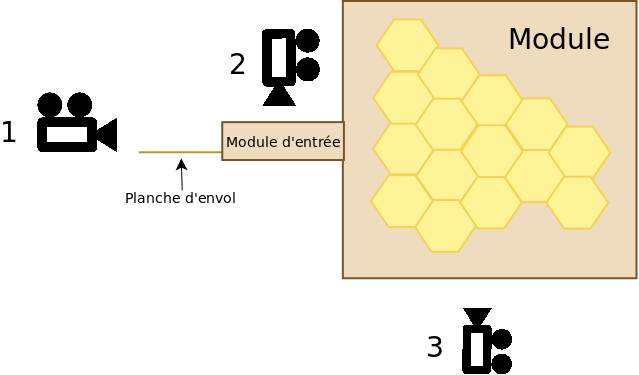
\includegraphics[scale=0.3]{../images/dia/schema_camera.png}
\end{center}
\begin{itemize}

  \item Les caméras situées sur la planche d'envol (1), tout d'abord, servent à surveillers 
  les alentours de la ruche. Elles permettent avant tout de
  mesurer le flux d'entrée/sortie des butineuses, mais également de détecter
  certains comportements, comme par exemple la ventilation forcée (une abeille
  bat des ailes afin de "pousser" de l'air frais vers l'intérieur de la ruche et faire
  diminuer la température ). Ces caméras vont aussi servir à mesurer la
  "pression" des prédateurs sur le rucher, en mesurant le nombre de frelons
  asiatiques en embuscade (vol stationnaire) et le nombre d'abeilles
  capturées. Ces caméras sont au nombre de deux, formant une paire
  stereoscopique afin de pouvoir effectuer des mmesures 3D. \\
  En annexe, un lien vers une vidéo prise par l'équipe au début du projet est disponible. 
  On peut y voir une planche d'envol filmée et passée au ralentis. \\ 
 
  \item Les caméras situées sur le module d'entrée (2), quand à elles, servent à étudier
  les pelotes de pollen ramenées par les butineuses afin de reconnaître les
  plantes utilisées par les abeilles. Ces caméras sont caractérisées par de
  fort grossissement et sont associées à des éclairages pilotés par ordinateur
  (UV, IR) pour mesurer l'autofluorescence des pollens.

  \item Enfin, les caméras montés sur chaque module (3) (1 par face du module) servent
  à détecter et surveiller les évenements qui ont lieu sur le couvain et sur
  les alvéoles. Ces caméras doivent travailler dans des conditions de lumière
  particulières, car la reine et certaines castes d'abeilles sont sensibles à
  la lumière visible. Pour ne pas les perturber, le rucher est placé en
  lumière rouge ou infrarouge, ce qui correspond à des longeurs d'onde que les
  abeilles ne voient pas. Il est a noté que des caméras supplémentaires,
  purement infrarouges, seront également utilisées dans le cadre des travaux de
  l'IES, l'un de nos partenaires.
\end{itemize}

  Les flux d'images générés par ces caméras sont collecté sur un réseau privé,
  puis transférés à un serveur central. En fonction du besoin, ils pourront
  etre enregistrés, renvoyés vers le site vitrine, renvoyées vers l'application d'annotation
  ou encore traités par les algorithmes qui sont mis au point par M. Triboulet et M. Druon. 
  Ces derniers se basent sur des réseaux de neurones afin de reconnaitres des comportements
  (danse, ventilation, etc) de facon automatique.


Au vu de la description générale de l'utilisation des vidéos ainsi qu'après discussion avec l'équipe, le logiciel devrait 
pouvoir permettre de : \\
\begin{itemize}
    \item Visualiser les caméras en direct
    \item Démarrer la capture vidéo à tout moment 
    \item Ajouter un système de tag par mots clés afin de pouvoir trier facilement les vidéos 
    \item Avoir plusieurs types d'annotations (entourer, marquer, avoir des mouvements etc) 
    \item Retrouver toutes les mesures de la ruches (température, horaires, numéro de caméra, de ruche, de cadre etc )  
    \item Avoir un principe d'auteur 
    \item Pouvoir revisualiser les vidéos 
    \item Pouvoir remodifier les vidéos 
\end{itemize} \\
Afin de répondre à ces besoins, nous avons imaginé l'application suivante : 
\begin{center}
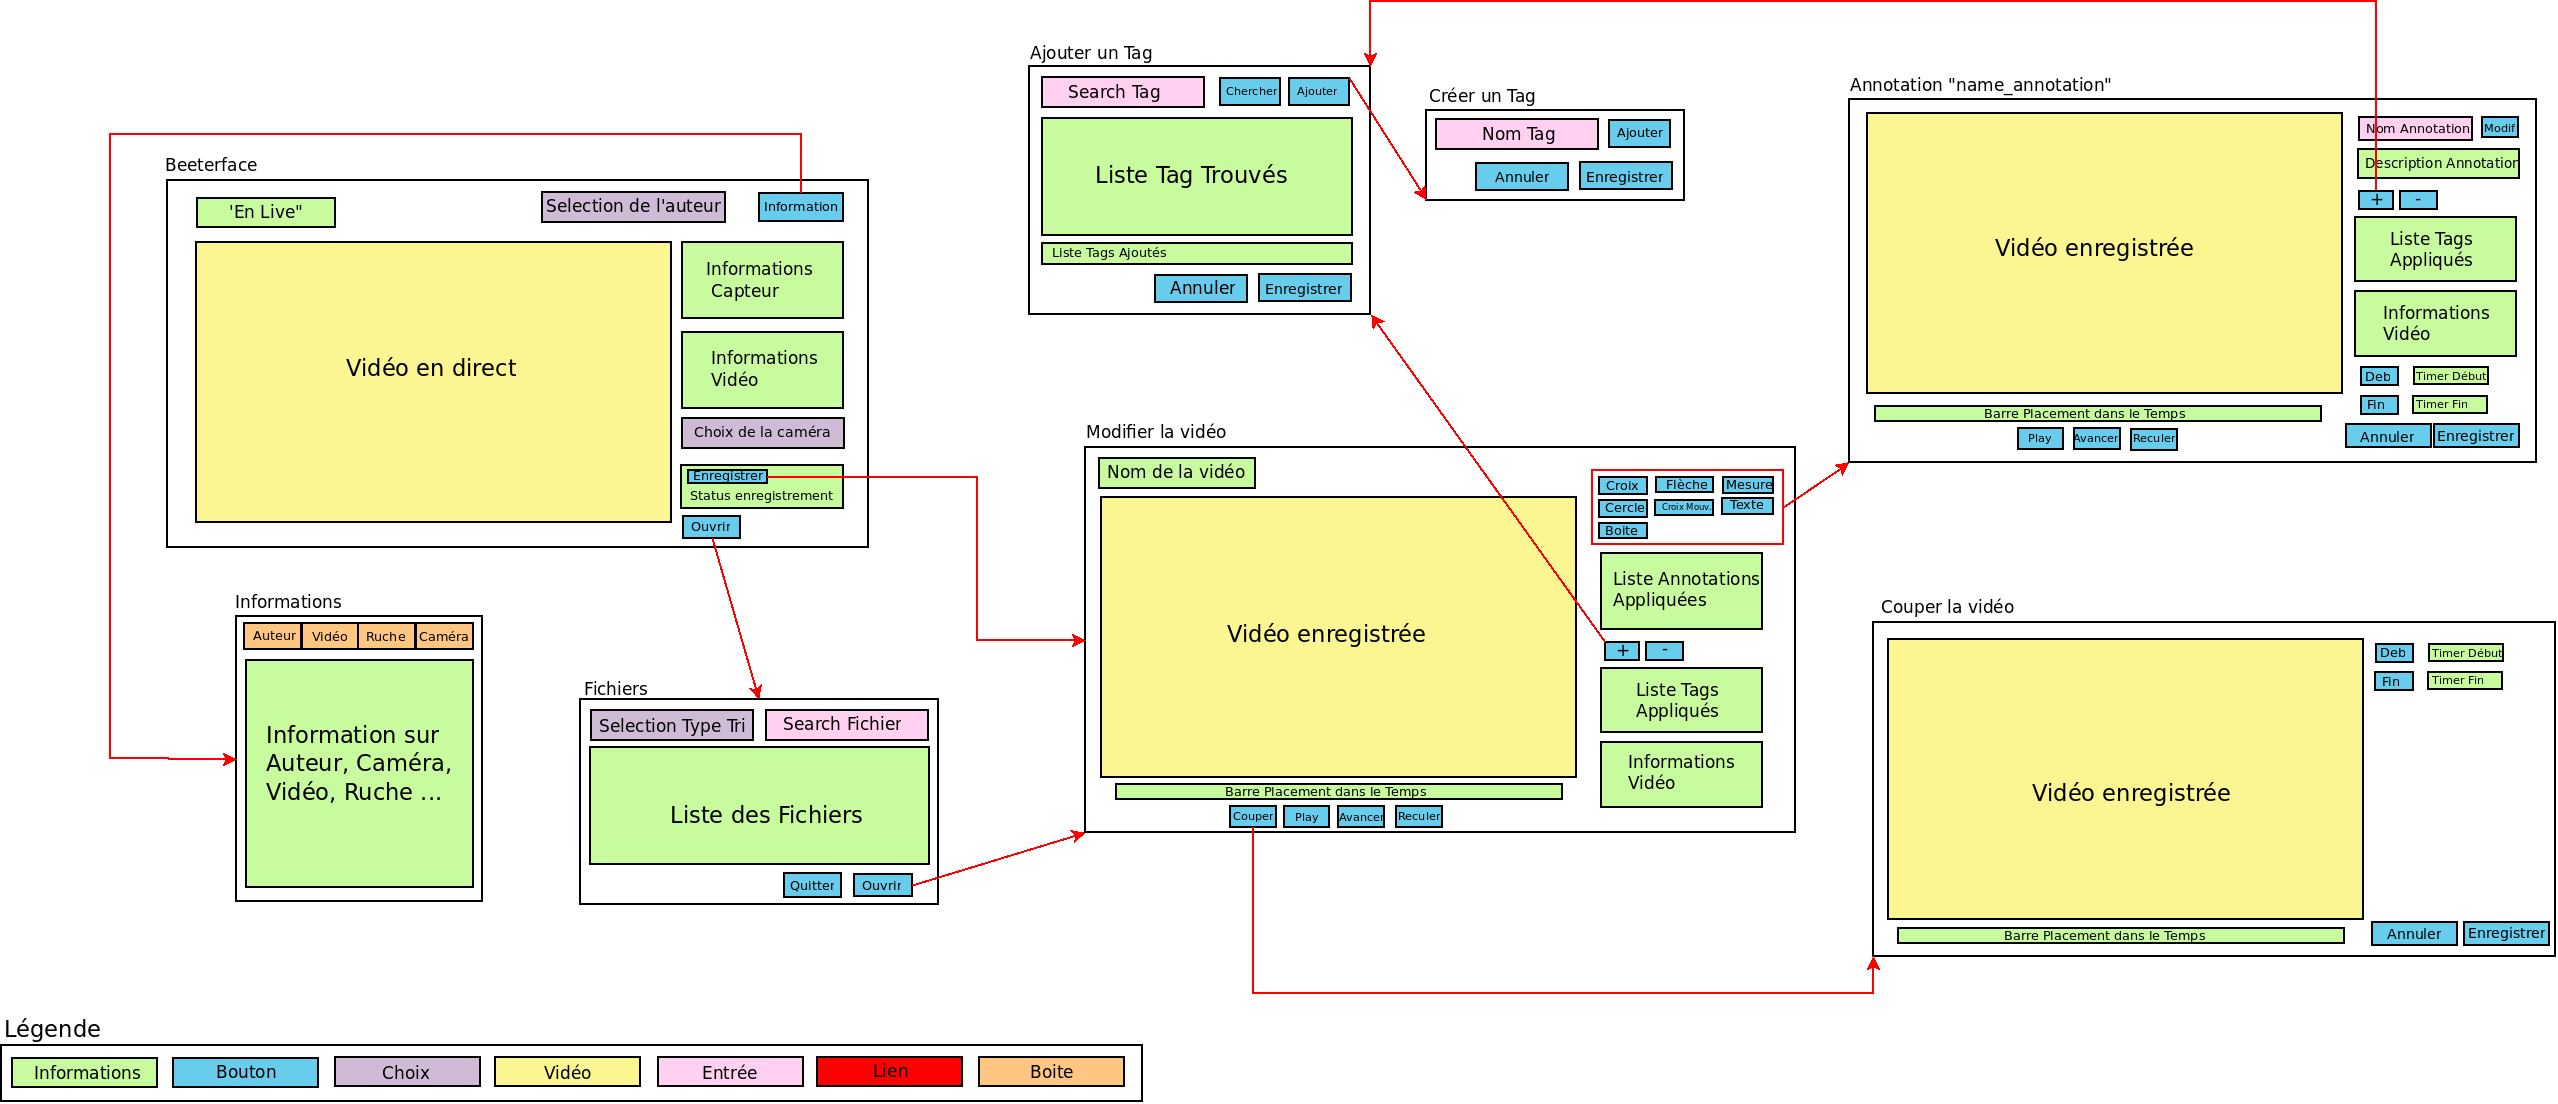
\includegraphics[scale=0.21]{../images/dia/schema_interface.png}
%TODO Intégrer la description bloc par bloc de win_main. Penser à essayer une mise en page par COLONNE 
\end{center}
    
Bien sûr, celle-ci a connu beaucoup d'évolutions au cours de son développement : au fur et à mesure de l'avancement,
nous nous rendions compte de certaines éventualités que nous n'avions pas imaginé et que nous avons intégré à la volée. 
Ainsi, ce schéma correspond à l'application actuelle mais n'avait pas été vu comme tel au début. 
\\

    \section{Contraintes} 
Le langage de départ pour coder l'interface et ses fonctionnalités, que nous pourrons familiairement nommer partie moteur 
et partie physique, m'a été imposé. \\
C'est donc en C que j'ai dû réflechir à comment préparer et lier ces deux parties. Ce langage a été choisit tout simplement 
parceque c'est  le langage que M. DRUON a pour habitute d'utiliser pour ce type de projet. \\
La partie moteur peut être développée en C sans trop d'ajout de librairies annexes autres que celles dites basiques 
(stdlib, stdio). 
Cependant, nous avons dû utiliser une librairie pour développer la partie physique. Nous pouvions utiliser GTK ou QT. 
QT devant être utilisé en C++, notre choix s'est naturellement dirigé vers GTK 3.0. \\
Comme dans tout projets collaboratifs, la convergence des données est importante et peut parfois se réveler difficile à mettre en place. 
Heureusement pour nous, en programmation l'outil GIT est excellent pour travailler à plusieurs. L'ayant déjà vu en cours cette année,
j'ai pu l'utiliser concrétement lors de mon stage. Cependant, avant de commencer à utiliser l'outil, il a été préférable que 
je me remette à niveau sur celui-ci et ai donc entammé la lecture du livre Mastering Git %TODO VERIFIER LE TITRE
qui m'a été d'une grande aide pour avoir des bases solides. Pour héberger notre code, nous avons choisi de le déposer sur GitHub : 
il est donc accessible au public sous le nom "superbeelive". %TODO ANNEXE lien github 

Pour cela, le livre %TODO Integrer ref du livre 
m'a servi de référence de base quant à la manière de manier les éléments. Je me suis également aidée de divers tutoriels sur internet,
mais surtout de la document officielle de GTK. %TODO Lien biblio 
\\
Souvent, on a tendance à utiliser Glade, un logiciel permettant de créer une interface GTK avec des outils graphiques. 
Dans mon cas, je m'en suis surtout servie en tant que bibliothèque pour voir et tester certains Widgets ainsi que leur fonctionnement. 

Cet utilitaire, certes plus rapide à prendre en mains, utilise en sortie des fichiers XML pour décrire l'interface ce qui, 
au final, complique la portabilité de l'interface d'une version du logiciel à l'autre. \\ 
De plus, j'ai préféré apprendre à utiliser GTK en ligne de code "brutes". Plus fastidieu au départ, 
j'ai trouvé cela plus simple à la longue : je maîtrisais vraiment mes outils et apprenais plus rapidement à utiliser 
un nouvel élément de la librairie.  
%TODO : intégrer capture d'écran glade ? 

        \subsection{Principe de GTK}
Apprendre à utiliser GTK sera plus long si la programmation objet nous est inconnu. En effet, même si le C n'est pas un langage objet,
GTK lui, reprend les principes de la programation objet. Si vous êtes déjà familier avec ce type de langage, alors l'apprentissage
sera bien plus rapide.\\
L'idée principale de GTK est que l'on va ranger tous les éléments en fonction d'un autre élément, pour finir avec des sortes de poupées 
russes qui s'emboîtent et se rangent côte à côte pour donner un résultat final. Il exite une multitude d'éléments utilisables, 
appelés les Widgets. L'élément de base "widgets" contient des propriétés, pour créer d'autre type d'élément, les développeurs de GTK 
en ont ajoutés d'autres. 
Au fur et à mesure, ces ajouts de propriétés ont permit de créer toute sorte de Widget : des textes, des labels, des tableaux, 
des séparateur, des listes, des bouttons... 
Ces héritage et cette hierarchie des objets va nous construire un arbre d'élements, nous permettant de savoir ce que l'on peut 
faire avec nos Widgets en fonction de qui ils héritent : 
\begin{center}
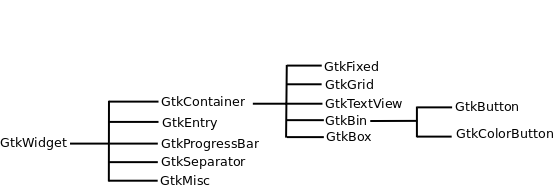
\includegraphics[scale=0.7]{../images/dia/arbo_widget.png} \\
\end{center}

En effet, si par exemple je veux changer un paramètre d'un élément "GtkSpinButton", et que je ne trouve pas de fonction 
affectant directement ce type d'élément, par exemple la taille, alors je vais regarder si chez ses parents je peux trouver 
le paramètre voulu, à savoir "GtkEntry", et "GtkWidget". \\

Chaque paramètre disponible pour les Widgets peut être changé directement à l'aide de fonctions retrouvable dans la très complète 
documentation en ligne de GTK 3.0. Il est totalement déconseillé de changer directement la valeur des paramètres à la mains 
en utilisant, par exemple des pointeurs. Il faut partir du principe que chaque élément a son nombre de fonctions associées 
et que tout est prévu pour pouvoir faire ce que l'on veut sur notre interface. \\ 
\\

        \subsection{Des boites, dans des boites...}
Une fois la manière de gérer les éléments et leurs paramètres acquise, il faut ensuite pouvoir les ranger. 
D'abord, on va créer une fenêtre, soit une "GtkWindow" que l'on va apeler Window. Dans celle-ci, on ne peut y poser qu'un seul Widget. 
C'est pour ça que nousavons les éléments "GtkContainers" : c'est avec eux que nous allons pouvoir structurer et placer tous les autres éléments 
comme on le veut dans notre fenêtre. \\

Le container de base est la "GtkBox". A sa création, nous devons simplement indiquer si celle-ci va être horizontale ou verticale, 
c'est à dire si les éléments que nous allons mettre dedans vont être placé de haut en bas ou de droite à gauche. 
Une fois cette première "GtkBox" placée, le problème de limitation de place imposée par la "GtkWindow" n'en est plus un. 
Maintenant, nous pouvons ranger ce que nous voulons dans cette boite. C'est là que le système de poupée russe prend son sens : 
nous allons devoir jouer avec les différentes boîtes pour créer les espaces que nous désirons. Voici le schéma de construction 
que j'ai fais pour la première fenêtre de l'application : \\
\begin{center}
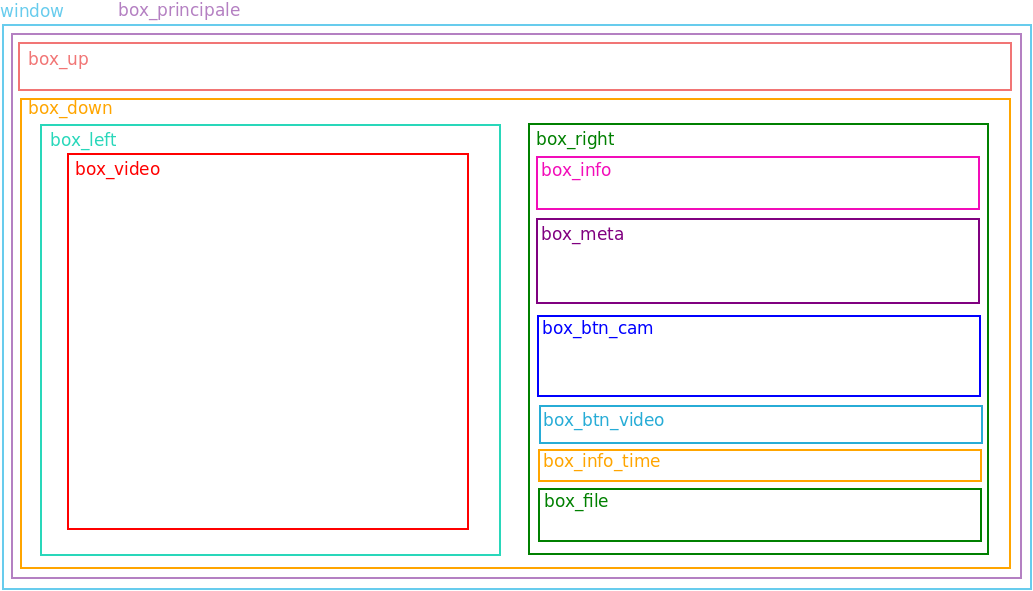
\includegraphics[scale=0.5]{../images/dia/schema_bloc_mainwin.png} \\
\end{center}

On peut voir que la GtkBox box\_principale prend toute la place de ma fenêtre GtkWindow. Dans cette box\_principale, j'y ai rangé 
verticalement box\_up et box\_down. Dans box\_down j'ai integré box\_left et box\_right horizontalement, me permettant d'avoir 
quatre zones délimitées. \\
Ensuite, j'ai créé des box pour mes éléments plus précis : dans box left j'ai directement intégré box\_video dans laquelle 
se trouve la vidéo (pour le moment, une image fixe représentant là où la vidéo se trouvera par la suite). 

Dans box right on va retrouver box\_info, box\_meta, box\_btn\_cam, box\_btn\_video, box\_info\_time et box\_file. 
Chacune de ces box m'ont permit de ranger à l'intérieur les éléments que je voulais retrouver : 
les boutons, les textes, les descriptions etc. 

A noter qu'en plus de ces "GtkBox" j'ai également utilisé d'autres type de "GtkContainer", comme des "GtkFrame", l'encadrement
avec un titre autour de "Informations Capteurs" et "Informations Vidéo" ou des "GtkGrid", permettant de placer les éléments 
à la maniètre d'un tableau sans les bordures, ici utiliser pour les les lignes dans les deux encadrés "Informations". \\
Un autre type de Gtkcontainer intéressant que je n'ai pas utilisé ici est le "GtkScrolledWindow". Celui-ci permet d'ajouter
une barre de défilement afin d'afficher plus d'informations. \\

Le résultat nous donne l'impression de ne pas voir toutes les boites clairement : \\

\begin{center}
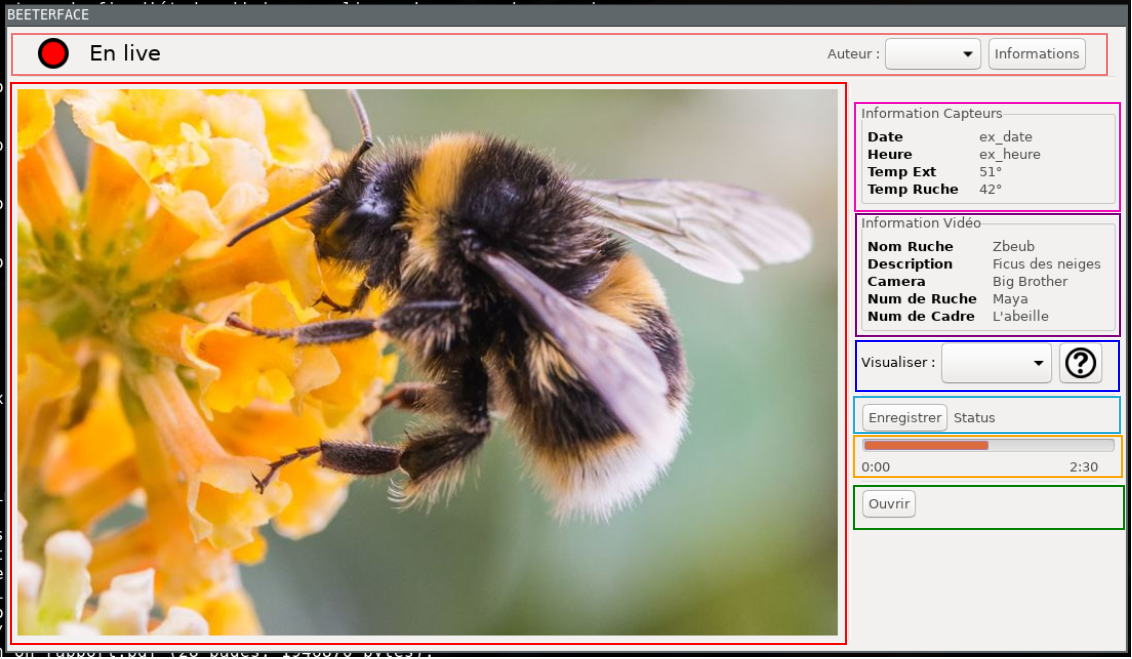
\includegraphics[scale=0.45]{../images/dia/schema_bloc_win_applique.png} \\
\end{center}

C'est dû au fait que les boite prennent toute la place qu'elle peuvent en fonction des widgets qu'elles contiennent. Ainsi, box principale 
n'est pas clairement visible : elle ne sert que de support pour celles qu'elle contient. 

Maintenant que nous avons tous les deux principes de bases en tête, à savoir les éléments et les boîtes, on peut voir comment 
tout cela se forme dans le code. \\

GTK nécessite une organisation rigoureuse si on veut pouvoir s'y retrouver avec les éléments rapidement nombreux.
Ainsi, j'ai voulu identifier les différentes étapes de la création d'un Widget et les séparer en 
trois grandes parties pour m'y retrouver plus facilement. \\

        \subsection{Création et Définition}

La première partie est la déclaration d'un Widget et sa définition. La création est simplement la déclaration de la variable 
avec son type. A noter que j'utilise des pointeurs pour toute mon application et que mes exemples 
sont inspirés des fichiers win\_main.c et win\_main.h afin que vous puissiez vous y reporter pour voir des exemples plus complets et
concrets. 
La structure en .c/.h et l'explication des pointeurs utilisés est décrite dans la partie "Les structures" de 
"Définition des fonctionnalités". Pour le moment, ne prenons pas en compte les "tmp" placés devant les noms des éléments. \\

Créons une fenêtre, une box et un label : \\

Dans win\_main.h : 
\begin{lstlisting} [frame=single]
GtkWidget* window ; 
GtkWidget* box ;   
GtkWidget* label ;  
\end{lstlisting}

Pour cet exemple, les éléments sont tous du type GtkWidget, ce sera le cas pour la majorité de nos éléments lors de la 
déclaration.
Il arrive que, dans de rare cas, il soit nécessaire de les déclarer autrement : si c'est le cas, la documentation l'indiquera. \\ 


Ces trois éléments existent désormais, maintenant il faut les définir, c'est à dire expliquer de quel type de Widget il seront 
et leur donner leur propriétés. \\

Dans win\_main.c :
\begin{lstlisting} [frame=single]
tmp->window = gtk_window_new (GTK_WINDOW_TOPLEVEL) ;
\end{lstlisting}

Ici, on utilise la fonction "gtk\_window\_new" pour indiquer que "window" est une fenêtre qui s'ouvre en premier plan 
avec l'argument "GTK\_WINDOW\_TOPLEVEL". \\

Dans win\_main.c :
\begin{lstlisting} [frame=single]
tmp->box_principal = gtk_box_new( GTK_ORIENTATION_VERTICAL, 0) ;
\end{lstlisting}

Comme dit plus haut, à la création d'une "GtkBox" on indique d'abord si on veut que les éléments soient ajoutés verticalement 
ou horizontalement. Ensuite, le second argument permet de définir le nombre de pixel d'écart par défaut entre les éléments, 
ici 0px, donc ils seront collés l'un à l'autre.  \\
%TODO VERIFIER ARGUMENT  !!

Dans win\_main.c :
\begin{lstlisting} [frame=single]
tmp->label = gtk_label_new("Je suis le texte du label") ; 
\end{lstlisting}
Enfin, le label nécessite lui aussi un argument, ici ce sera le texte noté de base. 
On peut laisser ce texte vide si on ne rempli pas les "".  \\


Les exemples ci-dessus ont tous eu besoin d'une définition précise du Widget, avec à chaque fois au moins un paramètre à régler. 
Il arrive parfoit que la création ne nécéssite aucun paramètre, et que des modification doivent être apportées ensuite. 
Par exemple, si je veux que mon label ai une écriture plus stylisée, je peux utiliser :  \\

\begin{lstlisting} [frame=single]
gtk_label_set_markup(GTK_LABEL(tmp->label), 
                    "<span foreground=\"black\" font=\"10\"><b>Je suis le label stylisée avec du bold</b></span>"); 
\end{lstlisting}

Ici, avant d'indiquer quel élément on veut modifier en argument, il faut préciser quel type d'élement c'est.
En effet, comme lors de la déclaration il est indiqué que label est de type GtkWidget et que la fonction que l'on veut utiliser 
ne s'applique que sur un GtkLabel, il est donc nécessaire de "forcer" GTK à considérer "tmp->label" comme un label.\\

Il existe plein de fonctions différentes permettant de régler ce genre de paramètres sur les widgets, et parfois il est nécessaire 
de faire appel à elles pour avoir un Widget correct. 
Il est intéressant d'explorer les fonctions existantes afin de personnaliser au mieux notre interface. \\

Une fois les Widgets créés, il faut maintenant les placer et indiquer qu'il faut les afficher. \\ 
 
\subsection{Placement, cosmétique et affichage} \\
Maintenant, nous allons appliquer la théorie qui avait été développée au dessus : les poupées russes. On va commencer par dire où 
va se placer la "GtkBox" : \\

\begin{lstlisting} [frame=single]
 gtk_container_add (GTK_CONTAINER (tmp->window), tmp->box) ; 
\end{lstlisting}

GtkWindow hérite de GtkContainer, nous utilisons donc la fonction qui permet d'affecter un élément à un container. Le premier argument 
indique le container où nous devons insérer un élément. Le second nous indique quel élément est à placer. \\

Ensuite, nous faisons de même pour la box : \\

\begin{lstlisting} [frame=single]
gtk_box_pack_start(GTK_BOX(tmp->box_principal), tmp->label, FALSE, FALSE, 0) ; 
\end{lstlisting}

"box\_principal" étant de type GtkBox, nous utilisons cette fois la fonction qui lui est associée. 
Comme pour "window", il faut indiquer la boîte concernée par l'élément à ajouter, mais cette fois-ci trois autres arguments 
sont à renseigner concernant la manière dont les Widgets vont se comporter à l'intérieur de la box. \\ 

Il faut savoir que par défaut (donc que tout est sur FALSE), les box allouent la même place à tous les Widgets qu'ils contiennent
sans déborder sur le reste.\\

\begin{itemize}
    \item Expand : peut être TRUE ou FALSE. Permet aux widgets de prendre plus de place si besoin si réglé sur TRUE. \\ 
    \item Fill : peut être TRUE ou FALSE. Ne peut être actif que si Expand est aussi TRUE. Alloue la hauteur ou la largeur totale
        de la box, 
        celon si la box est une horizontale ou vertical. \\
    \item Padding : valeur numérique. Indique l'espacement en pixel (px) entre les widget que contient la box. \\ 
\end{itemize}

Les éléments sont maintenant placés. Afin d'avoir une relecture facile et pour savoir qui se trouve dans quelle box ou container, 
j'ai appliqué une indentation  qui m'est propre mais que je trouve plus lisible, voici l'exemple complet pour win\_main.c : \\

\begin{center}
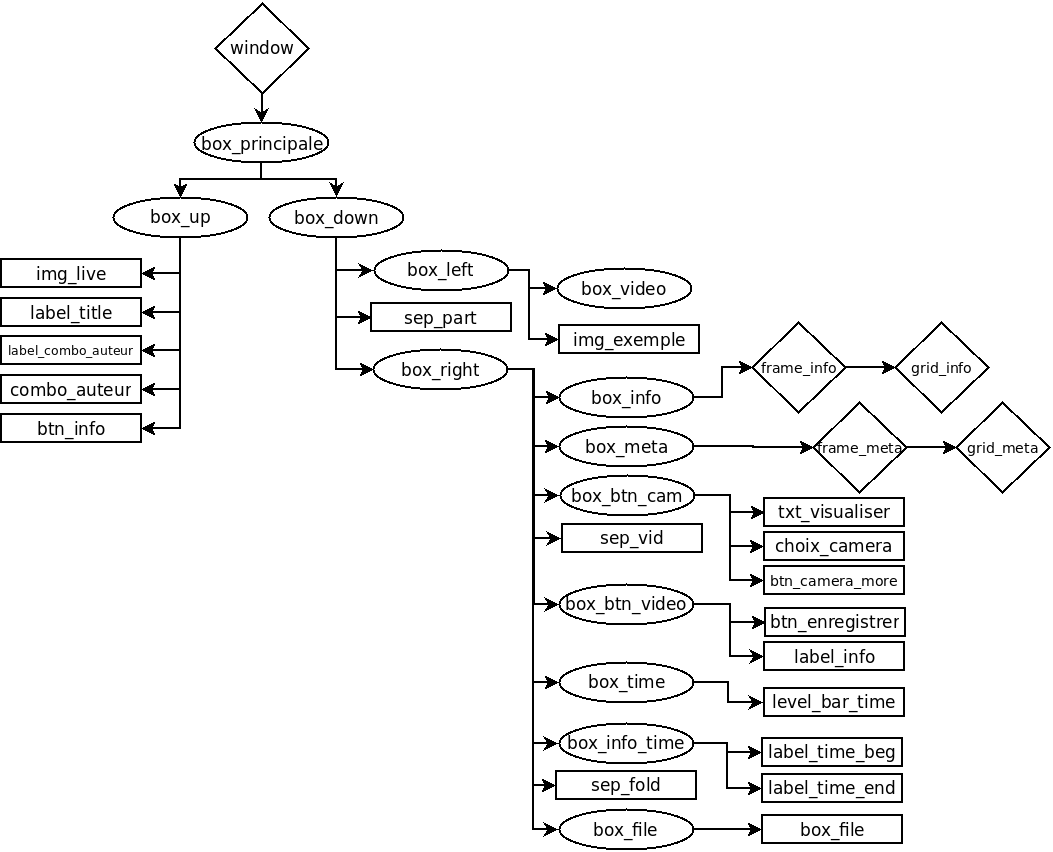
\includegraphics[scale=0.5]{../images/dia/diagramme_fenetre.png} \\
\end{center}
%TODO insérer ex de win_main   

Ainsi, à chaque fois que je vais dans une sous box, j'indente avec une tabulation. Au final, le rendu me permet de voir qui est
à quel niveau. \\
Petite précision, les éléments seront placés dans l'ordre de lecture du document. Ainsi, si votre "GtkBox" est créée en tant
que box horizontale, l'élément placés en premier sera le plus à gauche, le suivant à sa droite et ainsi de suite. \\ 


Une fois que les éléments sont placés dans les boîtes, ceux-ci sont tous collés les uns aux autres. Il faut indiquer 
comment ils doivent se placer. Pour mieux comprendre, voici un avant / après l'étape que je vais décrire : \\ 

%TODO image d'un avant après de main_win

Tout d'abord, commençons par jouer avec les paramètres EXPAND et FILL des "GtkBox". Ils permettent de définir quels éléments seront 
autorisés à s'agrandir en même temps que la fenêtre. Le mieux pour bien comprendre leur comportement, c'est de tester au fur
et à mesure les différentes combinaisons. \\

Comme pour la création et le placement, nous allons utiliser des fonctions pour indiquer ce que l'on veut faire avec les éléments.
Ce type de fonction est utilisée sur les éléments de types "GtkWidget", et donc applicable sur tous ceux qui en héritent. Voici les
deux fonctions et leur variables que j'ai le plus utilisé : \\


\begin{lstlisting} [frame=single]
 gtk_widget_set_margin_top (GTK_WIDGET (tmp->label), 5 ) ; 
\end{lstlisting}

Permet d'appliquer une marge sur le haut. On précise sur quel Widget l'appliquer puis la taille en px de la marge.\\
Cette fonction existe aussi pour bottom, end et start qui correspondent au bas, à la droite et la gauche du Widget.\\
%TODO schéma bottom etc

\begin{lstlisting} [frame=single]
 gtk_widget_set_halign ( GTK_WIDGET (tmp->label), GTK_ALIGN_START ) ;
\end{lstlisting}
Les éléments se mettent par défaut au centre de leur place disponible. Cette fonction permet 
de forcer un Widget à se placer autrement : ici, on force l'alignement horizontal (halign) à être en début de zone, 
soit à gauche (START). \\
%TODO schéma halign etc


On peut aussi retrouver des fonctions pour préciser le comportement de la fenêtre, comme : \\
 
\begin{lstlisting} [frame=single]
gtk_window_set_title (GTK_WINDOW (tmp->window), "BEETERFACE") ; 
\end{lstlisting}
qui permet de nommer la fenêtre "BEETERFACE". \\

\begin{lstlisting} [frame=single]
gtk_window_set_default_size ( GTK_WINDOW (tmp->window), 30, 30 ) ; 
\end{lstlisting}
Définit la taille minimale de la fenêtre, sachant qu'elle prend en compte la place nécessaire aux éléments pour pouvoir 
être placés et que si la taille indiquée est trop petite, alors la fenêtre prendra la place minimale possible 
pour afficher les éléments. \\

Avec ces outils et un peu de recherches sur la documentation en ligne, on peut maintenant créer n'importe qu'elle fenêtre 
comme on le souhaite. 

Attention, à cette étape nous avons juste définit l'interface. Il reste encore une étape pour pouvoir afficher les éléments, sinon
les éléments seront créés, placés... mais pas affichés ! 

Personnelement, j'aime la faire en deux étapes. D'abord l'affichage de la fenêtre avec : \\
\begin{lstlisting} [frame=single]
gtk_widget_show (tmp->window) ;
\end{lstlisting}

Puis de la box principale avec tout ce qu'elle contient : \\
\begin{lstlisting} [frame=single]
gtk_widget_show_all (tmp->box_principal) ; 
\end{lstlisting}

Sachant que l'affichage se fera dans l'ordre annoncé, si vous avez peur que le logiciel apparaisse "étape par étape", c'est à 
dire avec les éléments apparaissant au fur et à mesure laissant au début une fenêtre vide restant affichées quelques secondes, 
préférez mettre l'affichage de la box principale avant l'affichage de la fenêtre : ainsi, la box et ses enfants sera déjà générée 
et n'aura besoin que de son support. Cependant, cette question se pose uniquement si l'application à afficher nécessite beaucoup de 
ressources. \\

Il ne reste plus qu'à lier des fonctions aux différents éléments pour que notre application soit 
fonctionnelle.\\
        
        \subsection{Signaux et fonctions} \\
Avoir des boutons, c'est bien. Pouvoir les utiliser, c'est encore mieux. Maintenant que tous éléments sont placés, 
il ne reste plus qu'à les lier aux fonctions qui permettront de réaliser diverses tâches (mettre en pause la vidéo,
se déplacer dans le temps de celle-ci, débuter la sauvegarde etc).    
C'est ce qui va établir le liens entre le moteur et la carcasse. \\

Pour le moment, peu de fonctions ont été écrites pour le moteur : toute la partie graphique est prête à les acceuillir 
mais le développement des fonctionnalités est ce qui prend le plus de temps. En guise d'entraînement et pour 
pouvoir être prête le jour où il faudra faire tous les liens, j'ai déjà fait quelques tests pour comprendre les principes. \\

Les liens entre l'interface et les fonctions vont se passer dans le main. Dans notre code, il est présent dans beeterface.c.\\

Avant tout, il faut noter que quelques fonctions de sont obligatoires pour pour le fonctionnement de GTK voici le modèle de base : \\

\begin{lstlisting} [frame=single]
int main(int argc, char *argv[])     
{ 
 gtk_init(&argc, &argv); 
 [votre code] 
 gtk_main();
 return 0 ;
} 
\end{lstlisting}
Les deux fonctions permettent d'initialiser l'interface et d'indiquer que celle-ci est en attente de signal
de la part de l'utilisateur pour réagir. \\

Maintenant que nous avons la base, commençons à intégrer des évenements. \\
Le but va être d'appeler une fonction GTK qui va lier un éléments à une autre fonction que nous avons écrit  (Callback) 
et d'indiquer en quelles circonstance la fonction doit réagir. Voici ladite fonction : \\

\begin{lstlisting} [frame=single]
g_signal_connect( queen->interface->win_main->btn,
                   "clicked", 
                    G\_CALLBACK(callback_btn) ,
                    queen ) ; 
\end{lstlisting}
Le premier argument correspond à l'élément qui est visé. Dans notre cas, beaucoup de pointeur sont en jeu,
pour le moment nous allons passer outre ces pointeurs : ils seront expliqués dans la partie structure. 
Partons simplement du principe qu'il faut appeler le bouton ou élément concerné.  \\

Le second argument sert à indiquer à quel évenement il faut réagir. Il en existe une liste prédéfinie : ici
c'est l'événement "clicked". Lorsqu'on cliquera sur le bouton, la connection sera établie. \\

Le troisième argument correspond à la "callback" appelée, soit la fonction qui doit se déclancher. Nous allons 
y revenir. \\

Le dernier argument indique ce qu'on envoit au callback comme information. Ici, c'est "queen", une sorte de 
gros paquet. Comme pour les pointeurs, ce sera expliqué plus tard. \\


Allons vois la callbak qui est appellée : \\

\begin{lstlisting} [frame=single]
void callback_quit_tag(GtkWidget* widget, gpointer data) {                                       
    queen_t* tmp ;                                                                             
    tmp = data ;                                                                                
    gtk_window_close (GTK_WINDOW(tmp->interface->win_main->window)) ; 
} 
\end{lstlisting}

Cette callback contient le strict minimum pour faire fonctionner simplement un bouton.\\
En arguments, elle reçoit d'abord le widget qui est à la source de son appel : dans notre cas, c'est "btn". \\
Ensuite, elle reçoit les data que "g\_signal\_connect" a envoyé, c'est à dire "queen". \\

Les deux premières lignes indiquent que la variable tmp reçoit les informations de data. \\
Enfin, la fonction utilisée permet d'indiquer qu'on va fermer une fenêtre, ici celle de win\_main, donc là où on
se trouve. Cet exemple est basique, on peut évidement faire bien plus et toucher à l'interface en elle même, déclancher
d'autres fonctionnalités, ouvrir de nouvelles fenêtres, modifier des informations...\\

Tous les outils principaux pour pouvoir créer une interface GTK ont été présentés. Avec ceux là, beaucoup de recherches
dans la documentation et le "catalogue" %TODO
de GTK, on a en mains une infinité de possibilité. Certaines actions nécessitent plus de reflexion que d'autre, mais 
au final ça n'est que de l'algorithmie ; toute la syntaxe est là. \\


    \section{Les fonctionnalités} 
        \subsection{Structuration du code}

La première chose que j'ai eu à faire pour la création de l'application a été de réfléchir à la façon dont elle allait fonctionner.

En étudiant la demande, une chose majeure en ressortait : il y allait avoir beaucoup de type de données à traiter et sauvegarder. \\
Si on lit la liste des besoins présentés dans la partie %TODO
on peut voir qu'il y a, entre autre, une notion d'auteur, de caméra, de vidéo et de ruche. Voici les différentes structures 
qui seront utilisées : %TODO RECUPERER TRAVAIL DE SEBEUH AVEC DIA

Afin de pouvoir manipuler de telles informations, j'ai créé une structure pour chacun des éléments nécessaires. \\
Ils contiendront chacuns des informations nécessaires à leur fonctionnement : dates, noms, numéro de téléphone, lieu, référence etc. \\

Par exemple, voici la définition d'une de ces structure : 
\begin{lstlisting} [frame=single]
\end{lstlisting}
%TODO intégrer une définition de structure (.h)

Pour chacune des structures, j'ai également préparé des fonctions permettant de manipuler les données.
En général, on y retrouve une fonction pour créer un élément (new\_element), une pour le supprimer (del\_element),
et un jeu de fonction pour modifier (set\_partie\_element) ou lire les données contenues dans l'élément indépendemment 
(get\_partie\_element). \\
Les voici pour la structure présentée en exemple : 
%TODO INTEGRER EXEMPLE 
\begin{lstlisting} [frame=single]
\end{lstlisting}


Cette préparation permettra de pouvoir utiliser ces données sans avoir à se soucier des pointeurs : tout est prêt, il n'y
a plus qu'à choisir comment on voudra modifier les données lors de l'utilisation du logiciel. \\

Cette préparation a aussi été faite pour toutes les annotations que nous pourrons intégrer sur les vidéos : 
les cercles, flèches, croix... \\

Pour le moment, toutes ces annotations ne sont pas prête. Mais les plus basiques, comme la croix, ont déjà leur structure de préparées.
Sa définition se fait avec un simple x et un y. D'autres nécéssitent d'autres indications, comme un angle pour la flèche
ou un tableau de coordonées pour la crois mouvante. \\

En plus des description des éléments, tous contiennent un champ nom, auteur, couleur, description, temps de début 
(quand il apparaît sur la vidéo) et temps de fin (quand il disparaît de la vidéo). 
On peut aussi faire mention du champ "tag[]" et "tag\_size" qui correspondront à une pile de tag qui sont affectés à l'élément. \\

Ces tags font parti des fonctionnalités les plus difficiles à mettre en place. Certes demandés par les biologistes, ils ne sont 
pas urgents pour le moment. Nous les avons défini sur papier mais pas encore mis en place. \\

Il y aura une liste de tags disponible, un dictionnaire, dans lequel les biologistes pourront 
ajouter facilement des nouveaux tags. Les tags pourront être affectés aux différentes annotations appliquées
à une vidéo, et cette vidéo héritera de ces tags dans sa description, nous permettant de trier et récupérer les vidéos 
en fonctions de ce qu'il s'y trouve. \\
Concernant sa définition, un tag sera décrit par une pile. À ce niveau, il reste encore quelques précision à apporter
avant de la coder. Cette tâche est pour le moment en attente dans notre TO DO LIST. 


Ce travail de préparation m'aura prit environ une semaines. Il a été difficile seulement au début : il fallait réfléchir 
à comment créer une structure correctement, penser à bien utiliser les pointeurs et gérer leur allocation de
mémoire. Une fois un premier modèle fait, les autres se faisaient de plus en plus vite. Utilisant l'éditeur de texte VIM, j'ai 
énormément utilisé les "rechercher / remplacer" pour travailler. \\
Ce travail, bien que fastidieux, m'aura permit d'appliquer concrétement l'utilisation des pointeurs, ce qui 
me manquait lors de mon arrivée en stage. \\ 

%TODO RELECTURE
        \subsection{Manière de coder}\\
N'ayant pas d'habitudes particulières en code, j'ai été conseillée quant à sa structure, afin qu'il 
soit facilement lisible. Ainsi, j'ai utilisé des couples de fichiers .c et .h me permettant de séparer 
la déclaration d'une structure et des fonctions ainsi que la définition de celles-ci. \\ 
%exemple d'un fichier .c et .h

De plus, M. DRUON a rapidement intégré un Makefile afin de nous éviter de compiler manuellement à chaque fois, passant 
ensuite à CMake pour générer le Makefile automatiquement ensuite. \\


Une fois cette façon de faire mise en place pour la partie moteur, j'ai voulu l'appliquer à la partie
graphique. Ainsi, un couple de .c et .h a aussi été créé pour chacunes des fenêtres, le .h contenant 
toutes les déclarations d'éléments sous forme de structure. \\
%exemple .c et .h POUR WIN

Dans le .c on retrouve la fonction de création de l'interface avec au début la définition de "tmp" qui correspond donc 
au "papier cadeau" contenant toutes les déclarations des éléments. 

C'est pourquoi nous avons vu sur les exemples plus haut 
que pour appeler un élément nous devions utiliser un pointeur comme "tmp->label". \\

Notre fichier .c contient alors de quoi créer l'interface, l'afficher et la supprimer, la suppression revenant à appliquer les 
Free  nécessaires. C'est pour cela que dans notre main on retrouve ces fonctions et que celui-ci est allégé. \\
\\

Jusque là, cette technique m'a permit d'avoir une structure de code agréable et ordonnée. Seulement, c'est arrivé au moment de 
faire les premier liens interface / fonctions qu'un autre problème s'est posé : comment pouvoir accéder à toutes les données
dont j'ai besoin lorsque j'utilise une callback ? 
Comme dit dans la partie 2.2.5, lorsqu'on appelle une callback quand événement est détecté, deux informations sont 
transmises à la callback : l'adresse du Widget et une data qui aura été définie avec la fonction "g\_signal\_connect". \\

C'est le choix de cette donnée qui nous a posé problème : quand nous avons commencé
à coder les fenêtre permettant la visualisation des données des auteurs, caméras etc, nous avions besoin d'envoyer la structure
de la fenêtre auteur par exemples mais aussi les informations de l'auteur, ne se trouvant pas dans les mêmes fichiers.  \\
La solution la plus simple était donc de refaire des "paquets" plus généraux : nous avons créé interface.c/h et projet.c/h, qui seront eux
même contenu dans queen.c/h. \\
Interface contient toutes les fenêtres possibles et a une fonction de créations de toutes celles-ci ainsi qu'une fonction de suppression, 
permettant de les créer au démarrage de l'application et éviter des chargement. La fonction de suppression nous assure d'éviter toute perte de mémoire.\\
Même principe pour le Projet : il contient tous les éléments permettant le fonctionnement moteur afin d'avoir la même facilité
d'utilisation que décrite pour l'interface. \\
Queen est le paquet général, il contient Interface et Projet. Son nom est en l'honneur de la reine des abeille : 
un paquet pour les gouverner tous ! \\
\\
Voici le schéma général, décrivant qui contient qui :%TODO
\\
Et voici un bout de code représentant ce qu'on peut faire avec les paquets : 

allback\_auteur(GtkWidget * widget, gpointer data)
 {
     queen\_t* tmp ;
     tmp = data ;
     // Remplissage de la fenêtre avec le contenu de auteur
     auteur\_win\_fill(tmp->interface->win\_auteur, tmp->projet->video->auteur ) ;

     auteur\_win\_show(tmp->interface->win\_auteur);
 }
 void callback\_auteur\_modify\_name(GtkWidget* widget, gpointer data) {
         queen\_t* tmp ;
         tmp = data ;

         if ( tmp->interface->win\_auteur->button\_modif\_1 == 0 )
         auteur\_button\_modify\_name(tmp->interface->win\_auteur, tmp->projet->video->auteur ) ;
         else
         auteur\_button\_modify\_ok\_name(tmp->interface->win\_auteur, tmp->projet->video->auteur ) ;
   }

\\
Dans cet exemple on retrouve la fonction "auteur\_win\_fill", fonction écrite dans win\_auteur\_callbacks.c et définie
dans win\_auteur.h. J'ai séparé les fonctions utilisées dans les callbacks afin de les retrouver facilement. \\

Voici donc comment le projet a été réflechi et construit. Normalement avec ces détails, un développeur qui voudrait reprendre
le projet pourrait le faire. Dans cette optique, nous avons également prévu d'utiliser %TODO retrouver le nom de l'utilitaire 
l'utilitaire ????? pour documenter le code, quelques exemples sont d'ailleurs déjà présents, mais la documentation 
complète n'était pas une priorité, c'est pourquoi cette tâche a été laissée en suspens. 
       
        \subsection{Traitement de la vidéo}
La partie la plus complexe de ce projet à mon avis est le traitement de la vidéo. Elle s'attaque à des sujets sur lesquels j'ai 
encore beaucoup à apprendre. C'est pourquoi durant le stage, c'est plus M. DRUON qui s'en est occupé. De mon côté, j'ai surtout
pris en compte ce qui allait être fait avec et ce que j'allais devoir prévoir au niveau de l'interface pour que cela fonctionne. \\

Globalement, l'idée de ce travail est dans un premier temps d'afficher la vidéo sur l'application grace à 
la librairie FFMPEG. Afin de me faciliter
le travail de lien entre les boutons et la vidéo, M. DRUON a prévu de créer plusieurs fonctions type, comme avancer la vidéo, la 
mettre en pause, la reculer, pour qu'ensuite elles soient affectées correctement à l'interface. \\

Dans un second temps, il faut pouvoir enregistrer la vidéo une fois qu'elle est annotée. L'idée est de faire en sorte que les annotations
soient des PNG appliqués au dessus de l'image et qu'ils soient transportés dans les mêmes flux que les flux vidéos. \\

Ce travail, bien qu'il a été commencé, devrait être fini aux alentours de Septembre, c'est pourquoi sa description ici
est surtout théorique. \\


        \subsection{Ce qui reste à faire}
Une application prenant du temps à être développée, il est normal que celle-ci n'ai pas été finie en 3 mois. Pour pouvoir se situer
dans l'avancement de ce projet, j'ai établi une liste non exhaustive de ce qui, à l'heure actuelle, resterai à faire : \\ 

\begin{itemize}
    \item Etablir le système de sauvegarde des données
    \item Configurer la façon dont les données seront envoyées sur le serveur (fréquence d'envoi, envoi automatique ou manuel etc) 
    \item Coder la façon dont les tags vont être  gérés pour le tri des vidéos 
    \item Continuer l'affichage vidéo
\end{itemize} 
\\
De manière plus personnelle, j'aurai également aimé pouvoir retravailler la structure interne de beeterface.c qui est, à mon sens,
un peu brouillon. \\
\\
Pour finir cette présentation de l'application, voici quelques screenshots du travail qui a été effectué.
Le travail fu long et n'a cessé d'évoluer : au fur et à mesure, j'aurai appris de nouvelles techniques, de nouvelles façon de faire 
et aurais profité de nombreux conseils d'un développeur sénior. \\


\chapter{Acquis et compétences}
    \section{Missions annexes}
        \subsection{Gestion du Réseau du Rucher}
Le projet se basant sur du traitement et de la récolte de données, une infrastructure réseau est à prévoir. Pour le moment,
nous avons surtout préparé le terrain.  \\
Les données seront récoltées au rucher, puis acheminées vers le serveur installé au CNRS. Ce serveur les stockera et les traitera, 
les envoyant à différents endroits celon le besoin : vers les applications Beeterface pour de l'annotation, vers la future vitrine Web
etc. \\
Seulement à mon arrivée il n'était pas encore raccordé au réseau : tout le long de mon stage,  nous avons dû attendre que
le CNRS nous installe la fibre. \\

Voici un schéma, certes basique, de notre infrastructure réseau prévue à ce jour \\.
%TODO SCHEMA DU RESEAU

Même si un biologiste annotait les vidéos avec Beeterface directement au rucher, les vidéos devront obligatoirement passer une première 
fois vers le serveur puis revenir au rucher. Ainsi, entre l'envoi de vidéos venant de caméras pouvant atteindre de hautes
qualités et la réception de ces mêmes vidéos, la bande passante et le matériel réseau installé sur place 
doivent pouvoir supporter de tels charges. \\

C'est pourquoi le technicien s'occupant de l'installation de la fibre devait connaître quel trafic était prévu de manière un
peu plus détaillée. Afin de répondre à cette question, nous avons effectué un récapitulatif des caméras prévues. 


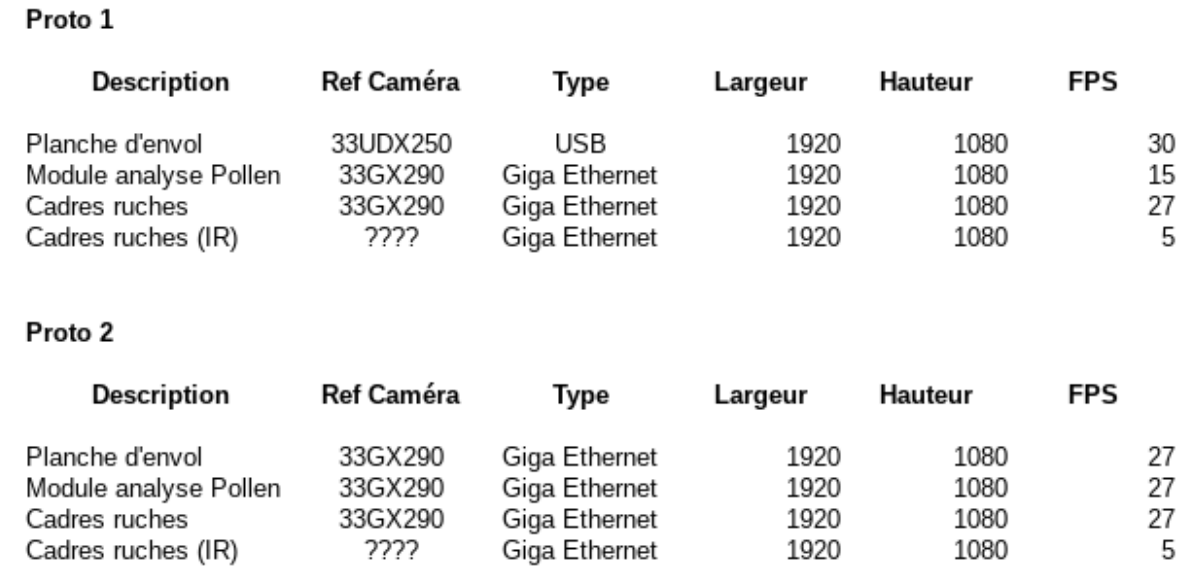
\includegraphics[scale=0.2]{../images/annexes/camera_bp.png} 

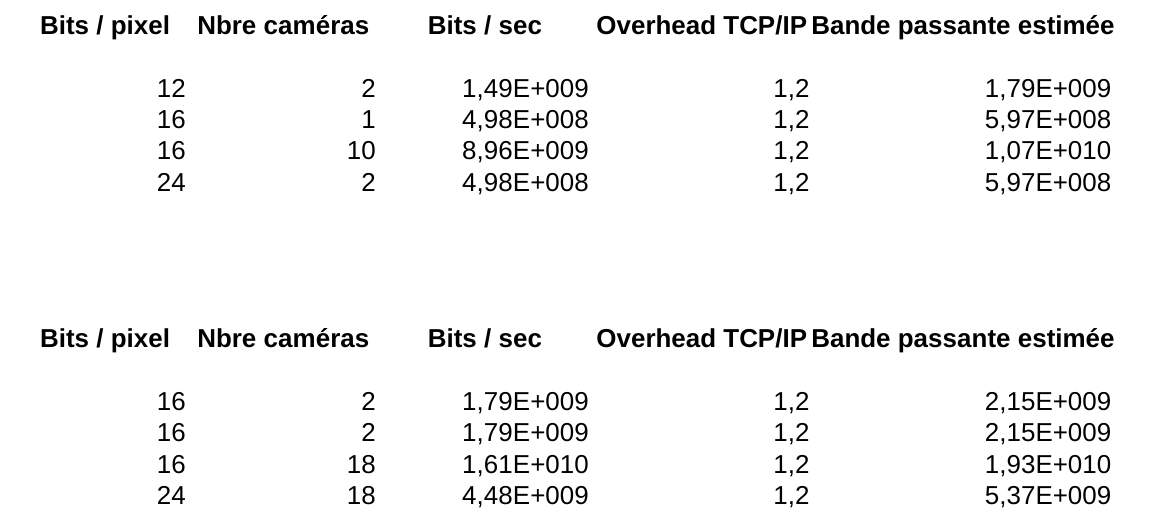
\includegraphics[scale=0.2]{../images/annexes/camera_bp2.png} 

Deux prototypes sont présentés, puisque nous comptons acceuillir deux prototypes de ruches plates : la notre et 
celle qui sera envoyées à nos partenaires Allemands ensuite. \\

Les caméras pour la planche d'envol et pour le module d'analyse de pollen seront en couleur. Celles pour les cadres de la ruches
seront monochrome : il avait été prévu des caméras couleurs à la base, mais d'après les biologistes nous en auront pas besoin pour 
repérer ce que nous voulons. Ainsi, nous gagnons en bande passante, les caméras monochrome étant moins gourmande que les couleurs 
en données. \\

En plus des caméras, il faut prévoir le poid des données des capteurs de la carte éléctroniques. Ces données sont négligeable par
rapport au reste mais sont à prévoir. Ces capteurs sont représentés dans le document par une des caméras "Cadres Ruches". 

Enfin, calculs prévoient également l'en-tête TCP-IP nécéssaire à l'envoie des données, cette prévision étant sur évaluée 
pour avoir de la marge. Ainsi, on ajoute 20\% de données supplémentaire.\\

Maintenant, nous savons un peu plus quels seront les données qui transiteront sur notre réseau. Nous avons aussi
quelques contraintes pour le choix du matériel réseau qui sera acheté dès que nous pourrons utiliser le réseau au rucher. \\
Le Switch servira à connecter les caméras, les capteurs, l'ordinateur déjà sur place et notre potentiel matériel supplémentaire
lorsque nous travaillerons sur place. Il devra être un 24 ports POE (Power Over Ethernet) capable 
d'alimenter nos caméra avec la norme SFP + requise par le technicien du CNRS. \\
Le serveur de récolte et de données devra être en double alimentation pour se suppléer l'une et l'autre en cas de panne,
assurant que le serveur tourne encore grace à la redondance. Il devra avoir un port Ethernet de 20Gb et posseder un CPU multicoeur.
Ce serveur doit être commandé chez DELL pour un budget de 15k€ maximum. \\
J'ai déjà fait quelques recherches sur leur site afin d'avoir une idée de ce qui existait mais la commande étant reportée à cause
du temps d'installation de la fibre au rucher, ces achats sont décalés à plus tard pour le moment.\\ 



        \subsection{Tests pour la vitrine Web}
En plus de l'installation réseau pour la récolte des données, il faudra aussi penser à comment nous allons présenter nos 
résultats. Ce travail servant de présentation, il est moins urgent que la réalisation des captures de données et à donc été mis de 
côté pendant mon stage. Cependant, j'ai passé une petite journée à me familiariser avec ce type d'installation en faisant 
quelques tests sur un serveur de test prêté par M. DRUON. Cette journée a surtout été consacrée à de la documentation en amont,
avec le lecture de quelques tutoriels sur Internet. J'en ai aussi profité pour relire les cours et 
TP du DUT en lien avec les serveurs Webs et le développement Web : base de donnée (M2104), langage HTML/CSS (M1106, M2105)
installation d'apache). 

Pour ce qui est du contenu de cette vitrine Web, je n'ai pas concrètement travaillé dessus mais ai imaginé à quoi celle-ci pourrait
ressembler. \\
%TODO schéma structure web simple  

Voici un schéma global de ce à quoi pourrait ressembler le site. Ceci n'est qu'une proposition qui n'a pas encore
été discutée avec le reste de l'équipe mais que je leur fourni. \\
Pour moi, le site pourrait être construit en quatre parties : 
- L'accueil, expliquant ce qu'est notre projet, qui en sont les acteurs
ce qu'on veut en ressortir etc. 
- La partie article, contenant des liens vers les publications faites par l'équipe concernant le projet, des articles écrits
spécifiquement pour le site ou des petit compte rendu d'avancement, avec des photos de nos opérations par exemple. Le but 
étant de montrer au public ce qui est fait et de rendre le projet attractif. Il faut que ce soit du contenu simple et rapide
à produire. 
- La partie Live, avec quelques caméras séléctionnées pour le grands public et la description des événements en temps réel par 
les algorithme qui seront réalisés par l'équipe. En attendant la réalisation de ces algorithmes, nous pourrions simplement afficher
le live de quelques caméras sans commentaires. \\
- La partie "pro", qui serait un portail de connexion pour les collaborateurs à qui nous voulons partager plus d'informations.
Ils auraient accès à plus de caméras, aux document techniques etc. On pourrait y mettre un drive afin de faciliter le partage de 
document. Ce serait une plateforme de travail pour le projet.\\

Bien sûr, l'élaboration d'un tel site nécessite des connaissances en web design et en sécurité informatiques. Je me suis penchée
sur la question parceque j'ai trouvé le sujet interessant et aimerai à l'avenir pouvoir m'y intéresser un peu plus. \\ 


        \subsection{Aide pour les projets de première année à l'IUT de Béziers}

En plus de mon aide sur les travaux cités si dessus, ma présence en tant que stagiaire a aussi été bénéfique pour aider M. Druon 
dans une tâche se détachant un peu du monde de la Recherche : aider durant les projets des étudiants en Réseaux et Télécommunications 
de première année. \\
Ce travail reste en lien avec SuperBeeLive puisque l'IUT de Béziers est partenaire du projet et qu'un des groupe d'étudiants (Groupe 13) 
a fait son projet sur la température et l'humidité dans la ruche. \\

C'est pour cela que durant toute ma durée du stage je me suis déplacée sur l'IUT de Béziers pour travailler les jeudis pour être
disponible, M. Druon et moi, pour les étudiants de RT1. Pendant ces jeudi ci, je travaillais le matin sur Beeterface et 
l'après midi je continuais de coder en salle projet pour répondre à d'éventuelles question. \\

J'ai également eu à m'occuper des commandes des étudiants : récolter leur liste de demande, les regrouper pour faire les commandes
aux fournisseur, réceptionner, inventorier et ranger. \\
%TODO Photo du rangement des commandes 

Ma présence sur l'IUT s'est intensifiée pendant les deux semaines où les étudiants étaient à temps plein sur leur projet, du 18 au 30 Juin. \\

Durant ces deux semaines, j'ai été affectée au bureau se trouvant à côté du laboratoire de l'IUT où j'avais rangé tous le matériel 
destiné aux projet.
J'ai donc servit de régie, car même après la première distribution du matériel demandé par les étudiants, beaucoup avaient 
besoin de pièce de rechange, de nouvelles pièces etc. \\

Cela m'a permit de continuer à travailler sur mon code, de manière moins intensive que lorsque je me trouvais au LIRMM, tout en
aidant M. Druon en le déchargeant des demandes de matériel. 
J'ai également aidé à noter les présences et ai fait attention au travail fourni par les étudiants afin de donner un avis extérieur pour
les notation.

Etant souvent dans les couloirs où ils travaillaient, j'ai aussi répondu à beaucoup de questions et demandes d'aide : 
j'essayai de répondre au mieux, de les diriger pour qu'ils trouvent la réponse d'eux même ou de les envoyer voir M. Druon si 
j'estimais que la question necessitait un oeil plus expert. \\

Au moment des soutenances, j'ai participé à un Jury devant normalement se tenir avec deux professeurs, mais M. Druon se retrouvant 
finalement seul dans celui-ci par manque d'effectif, c'est en binome que nous avons écouté le travail des étudiants.
D'autres deuxièmes années ou redoublant se trouvaient dans les trois autres jury avec d'autres professeurs. 

L'exercice de notation a été un peu difficile : bien qu'ayant un peu peur de noter injustement,
je savais très bien que la note qui allait être la plus importante serait celle 
du professeur. Néanmoins, c'était très interessant de se retrouver de l'autre côté et d'évaluer des travaux que, moi même, 
j'avais dû effectuer il y a un an. \\


Ces missions annexes m'auront permit d'appliquer concretement plusieurs notions vues pendant le DUT. \\
Théorique d'abord, avec les calculs pour la bande passant nécessaire pour le rucher et le questionnement sur le matériel à commander, ainsi
qu'avec les recherches autours du développement et l'installation web. 

J'ai aussi pu revoir beaucoup de sujets pratiques avec les étudiants de première année : beaucoup de leur question tournaient autours 
de choses que j'avais déjà fait, en cours ou en projet,  mais sur lesquels il me manquait expériences et connaissances à ces moments là et
qui ne me posent plus soucis aujourd'hui. \\


    \section{Compétences développées} \\

Lors de stage de fin d'étude, j'ai pu appliquer beaucoup de connaissances que j'ai acquises pendant ces deux dernières années,
mais aussi apprendre beaucoup à différents niveaux.\\

Mon rôle principal dans l'équipe n'étant pas de faire de l'administration réseaux et systèmes tous les jours, 
j'ai pu utiliser mes connaissances dans ce domaine d'une autre manière qu'en administrant des infrastructures déjà installées. \\ 
C'est surtout la théorie qui m'aura été utile, voyant plus le rôle d'un ingénieur que d'un technicien. 

Mes journées de travail se passant en grande majorité sur un ordinateur, j'ai au quotidien fais de l'administration Unix et ai
utilisé des outils que je ne connaissais que partiellement avant. Ainsi, mon but était d'être plus rapide avec ces outils 
et j'ai donc appris des raccourcis clavier et des techniques que me conseillaient les personnes autours de moi pour optimiser 
mon temps. \\

De plus, j'ai ensuite eu la chance d'avoir un ordinateur fourni par le LIRMM, également sous Unix.
Comme cette machine m'était destinée, j'ai pu passer du temps à la configurer comme je le voulais : 
installation d'une interface graphique (i3), configuration de VIM, d'un terminal personnalisé, personnalisation des couleurs 
sur mon shell, test d'une alternative à bash (fish) etc. 
Si je considère cette partie personnalisation, comme une compétence développée pendant le stage, c'est parceque j'ai eu la chance 
d'avoir autours une équipe pour qui il était important que je sois à l'aise avec mes outils de travails, me laissant une 
journée pour travailler là dessus. \\
Je pense ainsi avoir aujourd'hui bien plus d'aisance derrière une machine sous Unix qu'il y a 3 mois. \\


J'ai aussi beaucoup appris pendant les deux semaines d'encadrement d'étudiant. Même si je n'avais pas le statut de professeur 
ou de vacataire, ma place en tant que "seconde" de M. Druon auprès des premières années était bien ancrée 
et m'a permi de voir le nombre de compétences nécessaire pour faire un tel travail : patience, organisation, 
capacité à expliquer les concepts et endurance s'ajoutent aux connaissances nécessaire pour aider des étudiants. 


Enfin, les compétences que j'ai le plus développées sont bien entendu celles autours de la programmation. 
À mon arrivée dans l'équipe, je ne pensais pas que j'allais autant me consacrer au code : je n'étais pas très à l'aise avec ça 
pendant mes deux années de DUT et avais un peu peur de me lancer dans des projets d'envergures dans ce domaine. 

Mais une fois sur place et lancée, j'ai appris énormément en peu de temps. Je pense même pouvoir dire que j'ai rattrapé le retard 
que j'avais pris lors de mon DUT avec ces trois mois presque intensif sur le sujet. \\

J'ai bien mieux compris comment utiliser les outils de compilations et comment cette étape se déroulait. L'algorithmie m'est bien moins
effrayante, le langage C est devenu pour moi une référence et je continue d'en apprendre dessus régulièrement. 
Il ne me reste d'ailleurs plus qu'un pas avant d'attaquer le langage objet grace à GTK : cette partie de la programmation très graphique
me plaît énormément et c'est ce qui, je pense, m'a réconciliée avec la programmation. \\

Désormais, je travaille beaucoup avec GIT sur GitHub, en découvrant des projets disponibles dessus et en partageant mes scripts,
mes configurations Unix etc. 

En soit, j'aurai appris sur beaucoup de sujets différent, plus que ce que je n'aurai pu l'imaginer.
J'ajoute aussi qu'au moment où j'écris ces lignes, j'apprend à me servir de Latex, un langage de composition de document, 
puisque je rédige mon rapport de stage avec cet outils. 


\chapter{Conclusion}

Ces trois mois de stages auront été formateurs pour moi sur plein d'aspects. Ayant déjà connaissance du travail en entreprise depuis un an
avec un boulot d'été que j'avais eu dans une entreprise de développement logiciel, j'ai pu découvrir un autre milieu de travail : 
la recherche. \\
Dans ce cadre, notre équipe de projet était moins souvent réunies, vu que ce sont plusieurs laboratoires qui travaillent ensemble, 
mais elle n'en reste pas soudée et très agréable. Les trois personnes avec qui j'ai le plus eu de contact, Sébastien Druon, 
Capucine Carlier et Matthieu Rousset étaient tous trois présents à leur niveau pendant mon stage.  \\

%TODO FINIR CONCLUSION
\chapter{Annexes}
%        \begin{figure}[t]
%            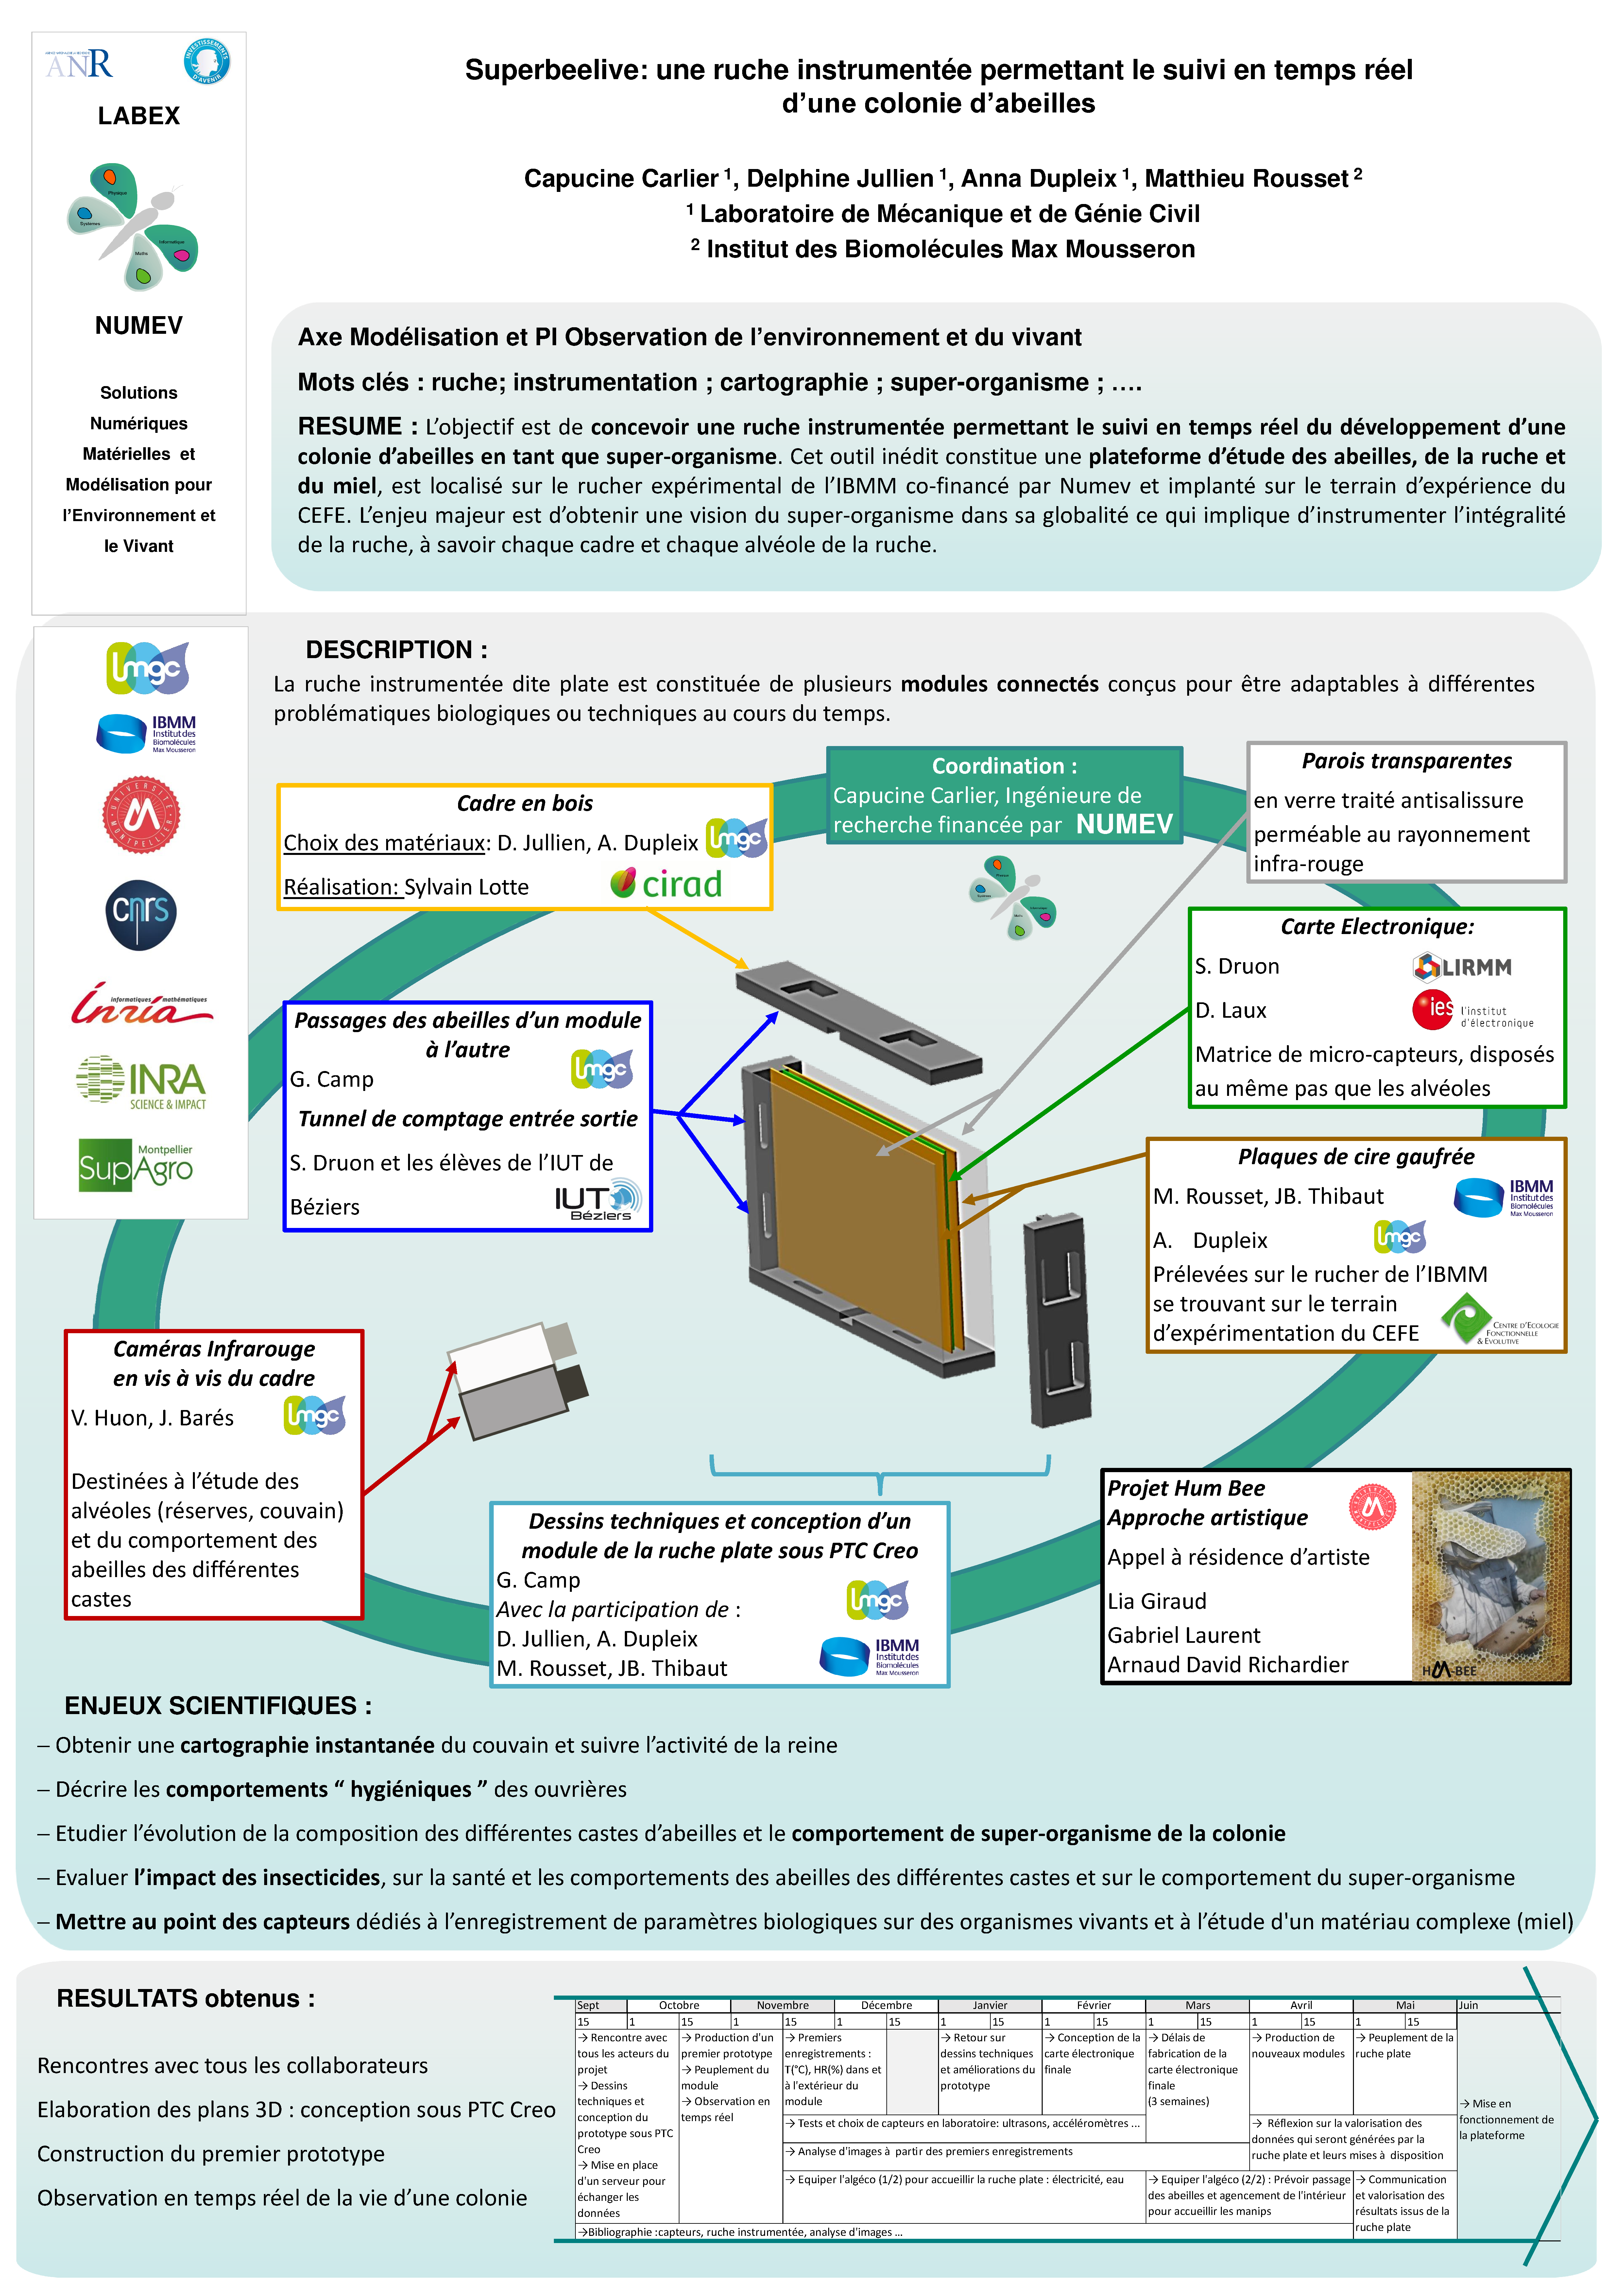
\includegraphics[scale=0.7]{../images/annexes/poster_numev.pdf}
%        \end{figure}
\end{document}





